% ****** Start of file apssamp.tex ******
%
%   This file is part of the APS files in the REVTeX 4.1 distribution.
%   Version 4.1r of REVTeX, August 2010
%
%   Copyright (c) 2009, 2010 The American Physical Society.
%
%   See the REVTeX 4 README file for restrictions and more information.
%
% TeX'ing this file requires that you have AMS-LaTeX 2.0 installed
% as well as the rest of the prerequisites for REVTeX 4.1
%
% See the REVTeX 4 README file
% It also requires running BibTeX. The commands are as follows:
%
%  1)  latex apssamp.tex
%  2)  bibtex apssamp
%  3)  latex apssamp.tex
%  4)  latex apssamp.tex
%
%\documentclass[%
 %reprint,
%superscriptaddress,
%groupedaddress,
%unsortedaddress,
%runinaddress,
%frontmatterverbose, 
%preprint,
%showpacs,preprintnumbers,
%nofootinbib,
%nobibnotes,
%bibnotes,
 %amsmath,amssymb,
 %aps,
%pra,
%prb,
%rmp,
%prstab,
%prstper,
%floatfix,
%]{revtex4-1}

%\usepackage{graphicx}% Include figure files
%\usepackage{dcolumn}% Align table columns on decimal point
%\usepackage{bm}% bold math
%\usepackage{hyperref}% add hypertext capabilities
%\usepackage[mathlines]{lineno}% Enable numbering of text and display math
%\linenumbers\relax % Commence numbering lines
%\usepackage{color}
%\usepackage{dsfont}
%\usepackage[showframe,%Uncomment any one of the following lines to test 
%%scale=0.7, marginratio={1:1, 2:3}, ignoreall,% default settings
%%text={7in,10in},centering,
%%margin=1.5in,
%%total={6.5in,8.75in}, top=1.2in, left=0.9in, includefoot,
%%height=10in,a5paper,hmargin={3cm,0.8in},
%]{geometry}

%\begin{document}

%\preprint{APS/123-QED}

%\title{Multi-dimensional optical trapping of a mirror}
%\title{Manuscript Title:\\with Forced Linebreak}% Force line breaks with \\
%\thanks{A footnote to the article title}%

%\author{Antonio Perreca}

% \altaffiliation[Also at ]{Physics Department, XYZ University.}%Lines break automatically or can be forced with \\
%\author{Second Author}%
 %\email{aperreca@syr.edu}
 %\author{James Lough}
 %\email{jdlough@syr.edu}
 %\author{David Kelley}
 %\email{dbkelley@syr.edu} 
%\author{Stefan W. Ballmer}
 %\email{sballmer@syr.edu}

%\affiliation{%
% Department of Physics, Syracuse University, \\
% Syracuse, NY, 13244 - 1130, USA }% \textbackslash\textbackslash}%



%\author{Charlie Author}
 %\homepage{http://www.Second.institution.edu/~Charlie.Author}
%\affiliation{
 %Second institution and/or address\\
 %This line break forced% with \\
%}%
%\affiliation{
 %Third institution, the second for Charlie Author
%}%
%\author{Delta Author}
%\affiliation{%
 %Authors' institution and/or address\\
 %This line break forced with \textbackslash\textbackslash
%}%

%\collaboration{CLEO Collaboration}%\noaffiliation

\date{\today}% It is always \today, today,
             %  but any date may be explicitly specified

%\begin{abstract}
%Alignment control in gravitational-wave detectors has consistently proven to be a difficult problem due to the stringent noise contamination requirement for the gravitational wave readout and the radiation-pressure induced angular instability in Fabry-Perot cavities (Sidles-Sigg instability).
%We present the analysis of a dual-carrier control scheme which uses radiation pressure to control a suspended mirror,
%trapping it in the longitudinal degree of freedom and one angular degree of freedom. We show that this scheme can control
%the Sidles-Sigg angular instability. Its limiting fundamental noise source is the quantum radiation pressure noise, providing an advantage compared to the conventional angular control schemes.
%In the appendix we also derive an exact expression for the optical spring constant used in the control scheme.
%\begin{description}
%\item[Usage]
%Secondary publications and information retrieval purposes.
%\item[PACS numbers]
% 04.80.Nn, 07.60.Ly, 95.55.Ym
%May be entered using the \verb+\pacs{#1}+ command.
%\item[Structure]
%You may use the \texttt{description} environment to structure your abstract;
%use the optional argument of the \verb+\item+ command to give the category of each item. 
%\end{description}
%\end{abstract}

%\pacs{Valid PACS appear here}% PACS, the Physics and Astronomy
                             % Classification Scheme.
%\keywords{Suggested keywords}%Use showkeys class option if keyword
                              %display desired
%\maketitle

\newcommand{\tcr}{\textcolor{red}}
\newcommand{\tcb}{\textcolor{blue}}
\newcommand{\tcm}{\textcolor{magenta}}
\newcommand{\tcg}{\textcolor{green}}
\newcommand{\tcp}{\textcolor{purple}}
\newcommand{\irm}{\mathrm{i}}

%\tableofcontents

\section{Introduction}
\label{sec:int}
%\section{\label{sec:level1}First-level heading:\protect\\ The line
%break was forced \lowercase{via} \textbackslash\textbackslash}

The Laser Interferometer Gravitational-wave Observatory (LIGO) is part of a world-wide 
effort to detect gravitational waves and use them to study the universe \cite{BPAbbott09}. Construction of 
LIGO's advanced detectors is underway. The installation is expected to finish in 2014. The goal of Advanced LIGO (aLIGO) is the first direct detection of gravitational-waves 
from astrophysical sources such as coalescing compact binaries and core-collapse supernovae.
These detections will open a new spectrum for observing the universe and establish the field of 
gravitational-wave astronomy. 
%The relatively weak coupling between gravity and matter allows 
%gravitational waves to penetrate domains unreachable by other forms of radiation. The universe 
%becomes opaque to photons and neutrinos at their respective cosmic surfaces of last scattering. 
%However gravitational waves can penetrate these barriers, and bring us information from the first 
%$10^{-43}$ seconds of creation.
These initial observations will also show the potential science gain of further increasing the state-of-the-art sensitivity of gravitational wave detectors \cite{Smith09,Harry10,Losurdo12}. Such detectors operate near the Standard Quantum Limit, meaning that the contributions from quantum radiation pressure and shot noise are about equal in the observation band \cite{Caves80, Ni86}.

To design a successor to aLIGO, techniques to operate gravitational-wave interferometers below 
the Standard Quantum Limit need to be developed \cite{Dan12, Chen13}. Dual carrier control systems and angular control 
using stable optical springs are promising methods for evading quantum-mechanical limitations on 
detector sensitivity \cite{LIGO10, Braginsky02b, Arcizet06b, Corbitt06b, Kippenberg05, Sheard04}. 
In 2007 Corbitt et al. at the LIGO Laboratory at the Massachusetts Institute of Technology 
demonstrated a one-dimensional optical trap of a one gram mirror using a novel two-carrier scheme \cite{Corbitt07}. 
%Although they did not completely turn off the low frequency feedback to the trapped mirror, 
Their work 
clearly demonstrated the potential of this technique. Extended to angular degrees of freedom, it has 
the prospect of opening a completely new approach to the angular control problem in future generation 
gravitational-wave detectors \cite{Punturo10}. 
Sidles and Sigg have shown that, for a Fabry-Perot cavity with a single 
resonating laser field, the radiation pressure force will couple the two end mirrors, always creating one 
soft (unstable) and one hard (stable) mode \cite{Sidles06}. This sets a lower limit on the required angular control 
bandwidth, which inevitably results in higher noise contamination by angular control noise and limits the angular control performance in the first and second generation 
gravitational-wave interferometers \cite{LIGO10, Braginsky01, Dooley13, Hirose10}. 
As we will show in section \ref{sec:IV}, angular optical trapping can bypass the Sidles and Sigg instability. Its fundamental noise limit is quantum radiation pressure noise, making it a promising candidate for low-noise angular control. Additionally, 
althoug we will not explore it in this paper, optical trapping of a mirror can be used to cool a mechanical degree of freedom. Depending on the mechanical system it can permit reaching the quantum ground state, enabling the manipulation of macroscopic object at the quantum level \cite{Teufel11, OConnell10, Chan11, TCorbitt07, Matsumoto13}. 

In this paper we present
a prototype of a position and yaw optical trap for a suspended test mirror using a double dual-carrier control 
scheme. 
We propose a system with two longitudinal traps acting on different spots of a single mirror; together, these traps will constrain both the position degree of freedom and one angular degree of freedom of the mirror.
This essentially replaces the current magnetic drives with optical traps.  The idea is promising and will be easy to apply to the other
angular degree of freedom.
The model includes two optical cavities with the trapped end-mirror in common. Each cavity is illuminated with two overlapping laser beams at different frequency detunings - one is positive detuned (blue detuning) and the other is negative detuned (red detuning).
The two dual-beams form two statically and dynamically stable optical springs with different lever arms and different power, designed such that the DC radiation pressure torques of the two dual beams cancel each other while 
DC radiation pressure force is canceled by displacing the position pendulum.
%comment from WARD:
%displaced from the center of the gravity of the test mirror; together, these constrain the relevant two degrees of freedom.  This is not unlike replacing magnet/coil actuators with optical traps.  It's a cool idea, and easily extensible.  

%Two pairs of carrier and subcarrier are created to form two optical springs both statically and dynamically
%stable. Radiation pressure forces associated at the two optical springs form torques in a way
%that they cancel to each other keeping the mirror trapped in its equilibrium. 
As a result, by picking the right 
parameters, we can obtain a system that is stable in the longitudinal and angular degrees of freedom with a mirror 
displacement range of the order of picometers.

The outline of this paper is as follows: In section \ref{sec:II} we review the idea of an optical spring. We then couple optical springs to a mechanical system and analyze the stability of the resulting opto-mechanical system.
Section \ref{sec:III} extends the stability analysis to more than one dimension.
In section \ref{sec:IV} we show that such a two dimensional optical spring is necessarily stronger than the Sidles-Sigg instability. In section \ref{sec:V} we calculate the radiation pressure noise, which is the fundamental limiting noise for radiation pressure control. Finally, in appendix \ref{app:A}, we derive the approximation-free expression for the optical spring in a Fabry-Perot cavity, which to our knowledge has not been published yet.

\section{Stability principle}
\label{sec:II}
%Firstly we consider the trap mirror as a suspended mirror located at the end of a Fabry-Perot cavity. 
%Dual carrier approach for mirror position control is based on the use of a strong (carrier) and a weak
%(subcarrier) field created to form two optical springs in such a way to have a stable system when 
%summed to the mechanical spring. %An additionally couple of beams need to be used for the angular control.

An optically detuned Fabry-Perot cavity naturally leads to a linear coupling between intra-cavity power and 
mirror position. Depending on the sign of the detuning, this coupling creates an optical spring which
is either statically stable or unstable. Due to the time delay in the optical field build-up, the optical spring 
restoration force is slightly delayed. This leads to a dynamically unstable spring for the statically stable case
and a dynamically stable spring for the statically unstable case. Corbitt et. al. \cite{Corbitt07} demonstrated that by adding a second, frequency-shifted optical field (sub-carrier) with a different detuning and power, a statically and dynamically stable optical spring can be achieved. The dual-carrier scheme has been used to optically trap a gram-scale mirror, controlling its longitudinal degree of freedom.
%thus creating an optical trap for the length degree of freedom of the mirror. 
Moreover, the damping of the optical spring can be controlled by adjusting the detuning of both carrier and sub-carrier and their relative amplitudes. This naturally allows for efficient cooling of the degree of freedom seen by the optical spring. In contrast to a mechanical spring, this damping does not introduce intrinsic losses, and thus does not contribute to the thermal noise.

This technique can be extended to alignment degrees of freedom. By duplicating the Corbitt et al. approach for trapping 
with a second, different, optical axis and a different beam spot on the controlled mirror, it is possible to control the angular 
degree of freedom with radiation pressure alone.
%, thus by-passing the Sidles-Sigg instability.

To be able to understand the stability of multi-dimensional opto-mechanical systems, we first recall the simple driven damped mechanical oscillator. From there we will stepwise increase the complexity by adding optical springs and additional degrees of freedom. 
%\tcr{Following we recall some of the features of a driven mechanical damped oscillator, we introduce the mathematical form of a optical spring and its relation with a mechanical oscillator in terms of control system model.}

%This lead us to the use of a two carrier scheme for the control of a single degree of
%freedom and to a double two carriers scheme for the control of two degrees of freedom.

%%%%%%%%%%%%%%%%%%%%%%%%%%%%%%%%%%%%%%%%%%%%%%%%%%%%%%%%%%%%%%
\subsection{Damped mechanical oscillator stability}
%%%%%%%%%%%%%%%%%%%%%%%%%%%%%%%%%%%%%%%%%%%%%%%%%%%%%%%%%%%%%%

Although the damped mechanical oscillator is a well known system, we will take it as a starting point to make the reading clearer. Our goal is to describe the mechanical oscillator in the language of control theory, which allows us to understand the stability of the system from a different point of view. This approach can then be naturally extended to include the effect of additional optical springs. 

The motion of a harmonic oscillator of mass $m$, spring constant $k_m$ and velocity damping $b$, driven by the external force $F_{ext}$, can be expressed as \cite{Saulson90}:
\begin{eqnarray}
\label{eqn:motion}
m\ddot{x}=-k_m x-b\dot{x}+F_{ext}
\end{eqnarray}
$b$ is also called the viscosity coefficient. Often the damping rate $\Gamma=b/(2 m)$ is used instead.
Traditionally the equation of motion \ref{eqn:motion} is directly used to get the system's position response $x$ when applying the external force $F_{ext}$. The resulting transfer function is
%For such a purpose and for completeness  we can describe the mechanical oscillator in two different way. 
%Both ways are self-consistent.
%One way is to consider the system as a mass with a mechanical spring that moves of the quantity $x$ when subjected at
%the force $F_{ext}$. The law that link the output $x$ and the input $F_{ext}$ of the system is
%given by the transfer function which can be directly obtained by the equation of motion (\ref{eqn:motion}):
%We consider such a system as free-test mass 
%\begin{figure}[htbp]
%	\centering
		%\includegraphics[width=6cm]{./images/Spring_add.eps}
%		\includegraphics[width=5cm]{./images/block_1.eps}
%	\caption{bla bla bla}
%	\label{cavity_k}
%\end{figure}

%That leads to the following transfer function:
\begin{eqnarray}
\label{eqn:TF}
G=\frac{x}{F_{ext}}=\frac{1}{-m\Omega^2+k_m+ib\Omega}                                                 %=\frac{1}{ms^2+b s+k_m}
\end{eqnarray}
with $\Omega$ being the angular frequency of the motion.
% and $s=i\Omega$ being a complex variable. % and $\Gamma=b/m$ is the damping rate. 

Alternatively we can describe a damped mechanical oscillator as a feedback system,  with the plant being just a free-test mass described by the transfer function 
$M=x/F_{ext}=-1/m\Omega^2$,
%Another way that can be used to describe a damped mechanical oscillator is to consider it as
%a feedback system where its plant is just a free-test mass described by the transfer function 
%$M=x/F_{ext}=-1/m\Omega^2$, 
obtained directly from the equation of motion of a free test-mass. 
The control filter of the feedback loop is the mechanical spring, which takes the mass displacement $x$ as input and acts on the plant with the control signal, or force, $F_K$, which is subtracted from the external force $F_{ext}$.
The transfer function of the control filter is $K_M=F_{K}/x=k_m+ib\Omega$. In this picture we can now calculate the closed loop transfer function and obtain the same expression as in equation \ref{eqn:TF}:
\begin{eqnarray}
\label{eqn:TF_fm}
G=\frac{M}{1+K_M M}=
%\frac{\frac{-1}{m\Omega^2}}{1-\frac{K_M}{m\Omega^2}}=
\frac{1}{-m\Omega^2+k_m+ib\Omega}
\end{eqnarray}
where $OL_M=-K_M  M = (k_m+ib\Omega)/m\Omega^2$ describes the open loop transfer function of the system.

%\begin{figure}[htbp]
%	\centering
%		%\includegraphics[width=6cm]{./images/Spring_add.eps}
%		\includegraphics[width=8cm]{./images/blocks}
%	\caption{{(Left)} A damped mechanical oscillator seen as system subjected to the external 
%	force $F_{ext}$ and corresponding displacement $x$ as output.
%	{(Right)} A damped mechanical oscillator seen as a closed-loop system, where the plant $M$
%	is a free-mass, the output is the displacement $x$ which is fed-back to the system through the elastic force $F_k= -K_M \cdot x$ and the input is $F_{ext}-F_{k}$.}
%	\label{fig:blocks}
%\end{figure}

\subsubsection*{Stability}
We can now check for the stability of the system in both pictures.
%The stability of the system related to the two different descriptions can be evaluated in a different manner.
%While the stability in the first description can be evaluated by looking at the poles of its transfer function, the latter
%offers the additional chance to look at its open loop transfer function $M\cdot K_M$ to evaluate its stability.
We recall from literature that the stability of a system described by its transfer function $G$ can be evaluated looking at the poles 
of its transfer function in the s-plane ($s=i\Omega$) \cite{Greensite70}. In particular a system is stable only if its transfer function's poles have
a negative real part,  and the multiplicity of poles on imaginary axis is at most 1.
The transfer function in equation \ref{eqn:TF} has the following poles:
\begin{eqnarray}
\label{eqn:poles}
i\Omega=-\frac{b}{2m}\pm\sqrt{\frac{b^2}{4m^2}-\omega_0^2},
\end{eqnarray}
where $\omega_0^2=k_m/m$ is the resonant frequency of the pendulum. 
%Comparing the damping rate $\Gamma=b/2m$ with the resonance frequency $\omega_0$ we understand the type of poles presents in $G$. If  $\Gamma>\omega_0$ then the poles are real and negative (over-damping), 
%if $\Gamma<\omega_0$ than the poles are complex conjugate at negative real part (under-damping),
%and if $\Gamma=\omega_0$ the system has two equal poles with negative real part (critically-damping).
The value of the damping rate $\Gamma=b/2m$ compared to $\omega_0$ determines whether the system is over-damped, under-damped or critically-damped. But since  $\Gamma$ (or $b$) is always positive, 
the real part of the poles is always negative. The system is thus always stable. 
%Here we want to point out that what ever cases we consider
%a damped mechanical oscillator shows poles with negative real component as $b$ and $k_m$ are in any cases positive, thus the system is always stable. 

From the control theory point of view, the stability can also be evaluated with no loss of generality by considering the open loop transfer function $OL_M= (k_m+ib\Omega)/m\Omega^2$ and applying, for example, the Bode stability criterion \cite{Franklin94}. The positivity of $b$ guarantees an always positive phase margin and therefore stability.
In the reminder of this work, for simplicity, we will test the stability of the control scheme using the Bode graphical method.

%as long as we consider the open loop transfer function $OL_M$. In this case the stability can be evaluated by using the %Nyquist criterion \cite{} by considering the plot of the open loop transfer function
%in the complex plane \cite{}

%can be evaluated by using the Nyquist criterion by considering the plot of the open loop transfer function
%in the complex plane \cite{}.


\subsection{Optical spring: a classical model}
Next, we look at an optical spring.
We start with a Fabry-Perot  cavity of length 
$L_0$, frequency detuning $\delta$, amplitude transmittance coefficients $t_1$, $t_2$  and amplitude reflectance coefficients $r_1$, $r_2$ of the input and output cavity mirror respectively. 
The light field inside the cavity builds up and exerts a radiation pressure force on both mirrors.
% In particular if  we calculate the power $P$ of the light inside the cavity, that can be  translated into radiation  pressure force exerted on the end cavity mirror.

We define the propagator $X=r_1r_2e^{-2i\delta\tau}$ and phase factor $Y=e^{-i\Omega\tau}$, with $\tau=L_0/c$ the one-way
travel time of the photon inside the cavity, $k$ is the wave vector of the light field  and $\Omega$ 
is the mechanical frequency of the pendulum. From this we can obtain an elastic force-law for small displacement values $x$, but potentially large detuning from resonance:
\begin{eqnarray}
\label{eqn:Frd}
F_{rad}=F_0-K_{OS}\cdot x + O(x^2),
\end{eqnarray}
where
\begin{eqnarray}
\label{KOS_full_2}
K_{OS}=K_0\left [ \frac{Y^2}{(1-Y^2X)(1-Y^2\overline{X})}  \right ]
\end{eqnarray}
%\begin{eqnarray}
%\label{KOS_full_2}
%\centering
%K_{OS}=-P_0 t^2 r_2^2 \frac{2ike^{-2i\Omega\tau}}{c(1-r_1r_2e^{ikL})(1-r_1r_2e^{-ikL})}\times\nonumber\\
 %\left( \frac{r_1r_2e^{-ikL}}{1-r_1r_2e^{-2i\Omega\tau} e^{-ikL}}-\frac{r_1r_2e^{ikL}}{1-r_1r_2e^{-2i\Omega\tau}e^{ikL}} \right) 
%\end{eqnarray}
is the optical spring constant and $\overline{X}$ is the complex conjugate of $X$. Here $K_0$ is the 
%static (frictionless) 
(mechanical) frequency-independent part of the spring constant:
\begin{eqnarray}
\label{eqn:K0}
K_0=F_0 \cdot 2 i k \cdot (X-\overline{X}),   \quad \mbox{with}\nonumber\\ 
F_0 = P_0 \cdot \frac{2  r_2^2}{c} \cdot \frac{t_1^2}{(1-X)(1-\overline{X})}
%K_0=\eta i \frac{X-\overline{X}}{(1-X)(1-\overline{X})}\quad \mbox{with}\nonumber\\ 
%\eta=P_0 t_1^2 r_2^2\frac{4 k }{c} 
\end{eqnarray}
The expression in equations \ref{KOS_full_2} and \ref{eqn:K0}
is the general expression for $K_{OS}$ up to linear order in $x$. While approximations for this formula have been published before \cite{Barginsky02}, we are not aware of a previous publication providing the full expression.
We address the complete derivation of the optical spring constant $K_{OS}$ in the Appendix \ref{app:A}. There we also show that with the approximations $2\Omega\tau\ll1$ and $2\delta\tau\ll1$  equation \ref{KOS_full_2} is equivalent to the expressions already existing in literature \cite{Barginsky02,Corbitt07}. 

We note that $K_0$ is a real number. Its sign is determined by the imaginary part of $X$. A positive sign is associated with positive detuning ($\delta>0$) and a restoring force (statically stable),  while a negative sign is due to  negative detuning ($\delta<0$) and
leads to a anti-restoring force  (statically unstable).  Also, for small (positive) frequencies $\Omega\tau\ll1$, the sign of the imaginary part of equation \ref{KOS_full_2} is opposite to its real part, leading to positive dynamic feedback for the statically stable case and  negative dynamic feedback for the statically unstable case.

Our next step is to couple the optical spring to a mechanical pendulum. We can treat this as either a damped mechanical oscillator with transfer function $G$, controlled by an optical spring $K_{OS}$, or as a free mass with transfer function $M$, controlled by the total feedback filter $H = K_M + K_{OS}$, see Fig.\ref{fig:blocks2}.
\begin{figure}[htbp]
	\centering
		%\includegraphics[width=6cm]{./images/Spring_add.eps}
		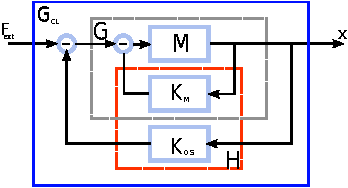
\includegraphics[width=15cm]{./figures/blocks_paper.pdf}
	\caption{{Mechanical oscillator and feedback systems. The mechanical oscillator can be seen as plant ($G$) and the optical spring $K_{OS}$ as feedback or
	alternatively as free test mass (plant M) and $H=K_{OS}+K_M$ as feedback. 
	Both the cases lead to the same closed loop transfer function $G_{CL}$ which describes the system as a damped mechanical oscillator in presence of
	the optical spring, subjected to the external force $F_{ext}$ and corresponding displacement $x$ as output.}}
	\label{fig:blocks2}
\end{figure}
In both cases we obtain the same closed-loop transfer function, equivalent to the one we would have obtained by
rewriting the equation of motion of a damped mechanical oscillator with an optical spring:
\begin{eqnarray}
\label{eqn:TFco}
G_{CL}=\frac{x}{F_{ext}}=\frac{G}{1+K_{OS} G}=\frac{M}{1+H M}\nonumber\\
=\frac{1}{-m\Omega^2+K_M+K_{OS}}%=\frac{1}{ms^2+b s+k_m}
\end{eqnarray}

The stability of the total system can again be evaluated  by either looking at the poles of the closed-loop
transfer function $G_{CL}$, or looking at the gain and phase margin of the open loop transfer function $OL_{MH}=-H/m\Omega^2$. The latter is generally more convenient. Unless compensated by large mechanical dissipation in $K_M$, the positive dynamic feedback for the statically stable case ($\delta>0$) leads to a dynamically unstable system. 
Intuitively this can be understood as a phase delay in the radiation pressure build-up which is caused by the cavity storage time.
For $\delta<0$ the system is statically unstable.

\subsection{Double Carrier Spring}

The seemingly intrinsic instability of optical springs can be overcome by a scheme 
proposed by Corbitt et al. \cite{Corbitt07}. The carrier is set at a large positive detuning ($\delta>0$, large $\delta/\gamma$). This provides a static restoring force, together with a relatively small dynamic instability (anti-damping). Then a sub-carrier is added at lower power and with a small negative detuning ($\delta<0$, small $|\delta|/\gamma$). The sub-carrier adds sufficient dissipation to stabilize the total optical spring, while leaving the sign of the static restoring force unchanged.
For appropriately chosen parameters of carrier ($c$) and sub-carrier ($sc$) (power $P_0^c$ and $P_0^{sc}$, detuning  $\delta_c$ and $\delta_{sc}$) the resulting total system thus becomes stable.

The spring constant of the total optical spring is simply the sum of the individual spring constants of the carrier and sub-carrier
\begin{eqnarray}
\label{eqn:KOSsum}
K_{OS}=K_{OS}^c+K_{OS}^{sc}
\end{eqnarray}
where the individual springs $K_{OS}^c$ and $K_{OS}^{sc}$ are given by equation \ref{eqn:TFco}.

%Fig.\ref{fig:stability} shows the stability of the trap-system at various values of  sub-carrier power and detuning for fixed carrier settings ($P_0^c=1~{\rm Watt}$, $\delta_c/\gamma = 2$) in our example system.

Conceptually we can think of the dual-carrier optical spring as a physical implementation of a feedback control filter for the mechanical system. With this tool at hand, we can start to analyze the behavior and stability of higher dimensional mechanical systems in the next section.

%\begin{figure}[htbp]
%	\centering
%		\includegraphics[width=9cm]{./images/KMKOSstability}
%	\caption{{Suspension stability region for different sub-carrier detuning ratio $\delta_{sc}/\gamma$ and input power values.
%	The carrier detuning ratio and its power have been set at $\delta_c/\gamma=2$ and $P0_c=1\,$W respectively. 
%	 At $\delta_{sc}/\gamma=0$ or $P0_{sc}=0\,$W only the carrier spring is effective and the system is not stable. The stability
%	 can be recovered only when the sub-carrier beam is injected into the cavity.}}
%	\label{fig:stability}
%\end{figure}


\section{Control model of longitudinal and angular degrees of freedom}
\label{sec:III} 

We will now extend our analysis to additional degrees of freedom. Experimentally, a torsion pendulum suspension is  easy to build. Therefore we will focus our attention to controlling the yaw motion of a test mirror, keeping in mind that the method can be applied to any additional degree of freedom. For actively controlling two degrees of freedom (length and yaw), we need a two-dimensional control system. In other words, we will need a second dual-carrier optical spring in a setup that for example looks like Fig.\ref{fig:angular}. We will label the two dual-carrier optical fields as beams $A$ and $B$. Each beam includes a carrier and a sub-carrier field, i.e.
\begin{eqnarray}
\label{eqn:beams}
\mbox{Beam A = carrier A + sub-carrier A}\\ \nonumber
\mbox{Beam B = carrier B + sub-carrier B}\nonumber
\end{eqnarray}
The two beams have a different optical axis, and each has its own optical spring constant, $K_{OS}^A$ and $K_{OS}^B$, given by equation 
\ref{eqn:KOSsum}.

If we define $x_A$ and $x_B$ as the longitudinal displacement of the mirror at the contact points
of beam A and beam B on the test mirror,
 %the position of the mechanical system at the attachment point of \tcr{incidence of} beam $A$ and beam $B$ \tcr{on the %test mirror}, 
 and $F_A$ and $F_B$ as the corresponding exerted forces, we can describe the mechanical system with a plant matrix $M$:
\begin{equation}
 \begin{pmatrix}
x_A\\ x_B
\end{pmatrix} 
=
M \begin{pmatrix}
F_{A}\\ F_{B}
\end{pmatrix}
\label{eq:MF}
\end{equation}
The explicit expression for $M$ for a torsion pendulum is given in appendix \ref{app:B}.

The control is provided by the optical springs. In the $x_A$-$x_B$ basis the control matrix $H$ is diagonal and given by  (also see Fig.\ref{fig:block_loops})
\begin{equation}
\begin{pmatrix}
F_{A}\\ F_{B}
\end{pmatrix}
= H
 \begin{pmatrix}
x_A\\ x_B
\end{pmatrix} 
=  \begin{pmatrix}
K_{OS}^A & 0 \\ 0 & K_{OS}^B
\end{pmatrix} 
 \begin{pmatrix}
x_A\\ x_B
\end{pmatrix} 
\label{eq:HX}
\end{equation}

\begin{figure}[t]
	\centering
		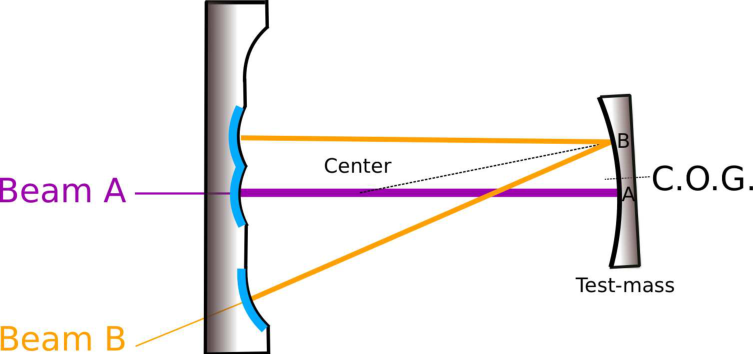
\includegraphics[width=15cm]{./figures/trap_drawing_paper2.pdf}
	\caption{
	In this sketch the main purple (Beam A) optical axis hits the test mirror %only slightly off-center 
	at point A, slightly displaced from the center of gravity (C.O.G.), such
	 that it still corresponds mainly to the length degree of freedom. Thus the second orange (Beam B) optical axis, which hits the test mirror closer to the edge at point B, needs much less power to balance the total DC torque. In our test setup the large input coupler is a composite mirror. It is 600 times more massive than the small mirror. The choice of a V-shaped beam B results in a more practical spot separation on the input coupler. }	


%with orders of magnitude more mass than the small mirror, 
%in order to ensure two different optical axes rigidly coupled.}	
	%can be as a multiple mirror.}%A monolithic, suspended platform is used for all auxiliary mirrors. %Once both one dimensional optical traps are engaged, i.e. their electrical feedback turned off, the DC alignment of the test mirror can still be adjusted by tuning \tcb{the...AOM frequency.}
	
	\label{fig:angular}
\end{figure}



\begin{figure}[htbp]
%	\centering
		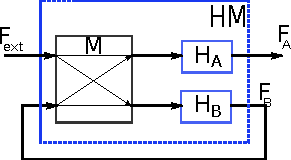
\includegraphics[width=15cm]{./figures/block_mimo_paper.pdf}
	\caption{Block diagram of beam A and beam B. The transfer function $F_A/F_{ext}$ is equal to $OL_A$ from equation \ref{eq:2dol}. Each loop affects the other resulting in cross terms
	present in the matrix $HM$. $M$ and $H_{A,B}$ are the transfer functions of the mechanical system and the optical springs of beam A and B, respectively.}
	\label{fig:block_loops}
\end{figure}

%\tcb{The model includes two optical cavities, referred to as beam A and B, both with an optical finesse of 104. 
%	The main cavity (beam A) is pumped with 0.8 Watt of carrier light, detuned by 36 kHz (blue detuning), and 0.2 
%	Watt of sub-carrier light, detuned by 12 kHz (red detuning). This produces a statically and dynamically stable 
%	optical spring with a lever arm of 1.3 mm, measured from the payload center of gravity. A second optical spring 
%	(beam B) is pumped with 16 times less power, but is otherwise similar to beam A. This side cavity has a lever 
%	arm of 2 cm on the payload, such that the DC radiation pressure torques of beam A and B cancel. The DC radiation 
%	pressure force is canceled by displacing the position pendulum.}

%\subsection{Method}
%\tcb{remove subsection}
For a multi-dimensional feedback system to be stable, it is sufficient that each individual (one-dimensional) feedback loop is stable, assuming all remaining control loops are closed. In other words, in our two-dimensional opto-mechanical system, we close the beam $B$ control filter for evaluating the open loop transfer functions $OL_{A}$, and vice versa. For the open loop transfer functions $OL_{A}$ and $OL_{B}$ we then find: 
\begin{eqnarray}
\label{eq:2dol}
OL_{A}=e_A^{T}\left(\mathds{1}-HM (\mathds{1} - e_A e_A^T) \right)^{-1}HMe_A  \\
OL_{B}=e_B^{T}\left(\mathds{1}-HM (\mathds{1} - e_B e_B^T) \right)^{-1}HMe_B \nonumber
\end{eqnarray}
with $e_A^T=(1,0)$ and $e_B^T=(0,1)$. The derivation of this expression is given in appendix \ref{app:C}.


%%%%%%%%%%%%%%%%%%%%%%%%%%%%%%%%%%%%%


\subsection{An Example}

It is worth considering a specific set of possible values for our model and evaluate the control of  angular and longitudinal degrees of freedom of a gram-scale test mirror using the radiation pressure of the light.
All the optical fields involved in our analysis are derived from the same wavelength light source through frequency shifting.
The model includes two optical cavities (Fig.\ref{fig:angular}), referred to as beam A and B, both with an optical finesse of  about $8000$ and linewidth $\gamma/(2 \pi) = 110\,$kHz. 
The main cavity (beam A) is pumped with $1\,$W of carrier light, detuned by $\delta/(2 \pi)= 250\,$kHz (blue detuning, $\delta/\gamma = 2$), and $0.2\,$W of sub-carrier light, detuned by $\delta/(2 \pi) =60\,$kHz (red detuning, $\delta/\gamma = -0.5$). This produces a statically and dynamically stable optical spring with a lever arm of $0.8\,$mm, measured from the payload center of gravity (C.O.G.). A second optical spring (beam B) is pumped with 6 times less power of carrier light, detuned by $=186\,$kHz (blue detuning, $\delta/\gamma=1.5$), and $40\,$mW of sub-carrier light, detuned by $60\,$kHz (red detuning, $\delta/\gamma=-0.5$). This side cavity has a lever arm of $3.3\,$mm on the payload, such that the DC radiation pressure torques of beam A and B cancel. The DC radiation pressure force can be canceled by displacing the position pendulum.

\begin{figure}[htbp]
	\centering
		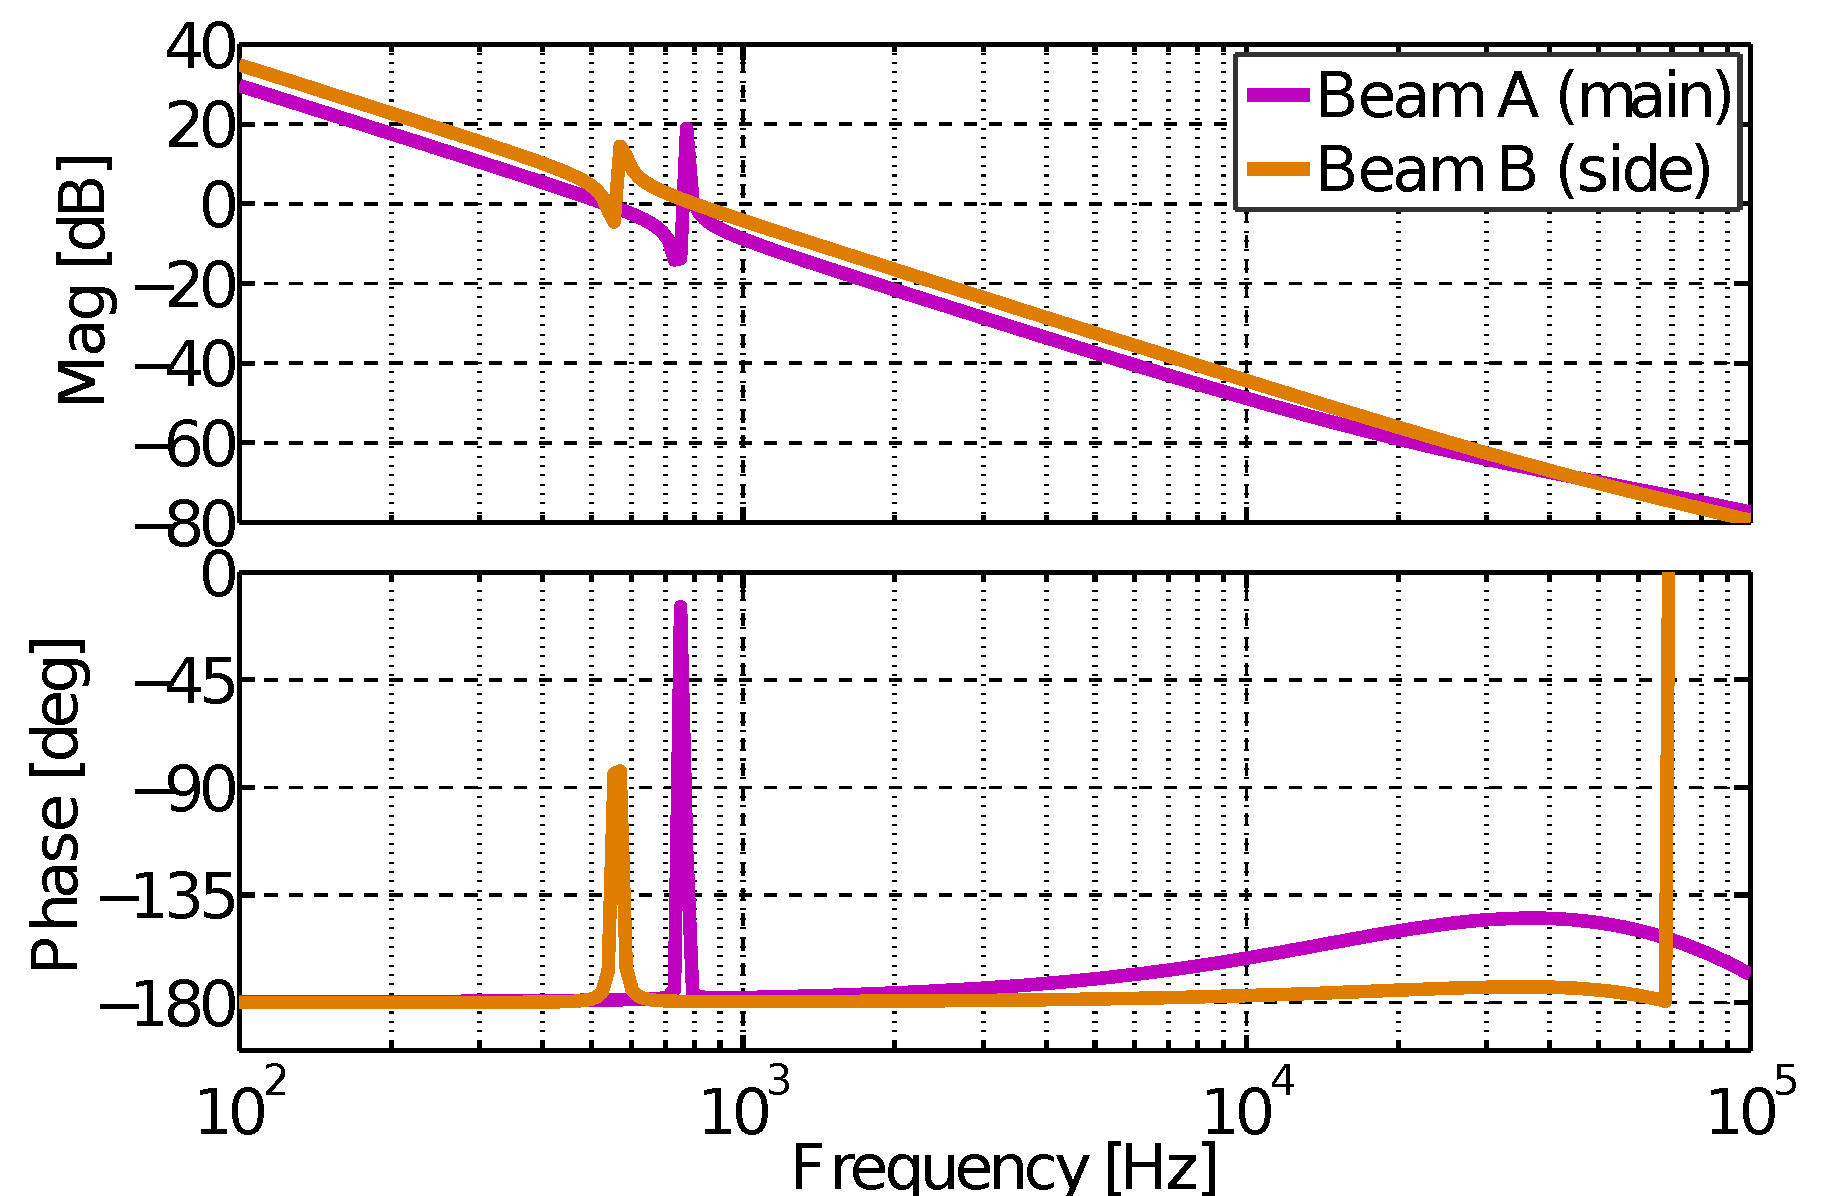
\includegraphics[width=15cm]{./figures/open_loops_TF_paper2.pdf}%filename.pdf}%
		%\includegraphics[width=8cm]{./images/filename.pdf}%
	\caption{{Open loop gain (OLG) for the main and side cavity.	The respective other loop is closed, and shows up as a resonance in the OLG. Note that, despite multiple unity gain crossings, both loops are stable because the resonances effectively implement a lead filter and the OLG avoids the critical point -1. Thus the dynamic interplay between multiple trapping beams on one payload does not introduce an instability.}}
	\label{fig:control_loops}
\end{figure}


The stability of the combined two-dimensional system is addressed in Fig.\ref{fig:control_loops}. Plotted are the open loop gain functions of the two degrees of freedom (the two optical traps) under the assumption that the other loop is closed. The presence of the second loop introduces a resonance feature in each loop at the unity gain frequency of the other loop. However the open loop gain avoids the critical point -1 (phase at zero), leading to a stable system. The model parameters were intentionally tuned for low damping / high quality factor in order to demonstrate that the system remains stable. Lower quality factors, and therefore stronger cooling is easily achievable.

%If we consider the cavity with both loops closed and we scan one of the mirror we obtain the stability region showed
%in Fig.\ref{fig:stability_region}. The green shaded area represents the offset range of the cavity length at which the two loops remain still stable. The range is $\backsim 20\,$pm.
%
%\begin{figure}[htbp]
%	\centering
%		\includegraphics[width=9cm]{./images/DC_offset}
%	\caption{{(Left) Static carrier and sub-carrier build-up as function of mirror position: Plotted are carrier and sub-carrier build-up (calibrated in Newton of radiation pressure) as a function of the respective cavity position. Also shown in blue is the total force. The trap is both statically and dynamically stable in the green shaded area.
%	%In Figure 4 the static (DC) radiation pressure force due to each of the four laser fields is plotted 
%%as a function of cavity position. Indicated by green shading are the regions with a stable optical 
%%spring (statically and dynamically). 
%With the chosen model parameters those regions are about 
%20 picometers wide.}}
%	\label{fig:stability_region}
%\end{figure}


\subsection{Stability range}
\label{sec:stability}
%\input{OT_paper_stabrange.tex}
We can now estimate the robustness of our feedback control system 
by changing the microscopic length $\delta x_A$ and $\delta x_B$ of the two cavities. This changes the detuning of the optical springs for both beams. Therefore the propagators $X_A$ and $X_B$ for both beams change according to $X_{A,B}=r_1r_2 e^{-i\delta_{A,B}\tau_{A,B}}\cdot e^{ik\delta x_{A,B}}$. For each position both the static and dynamical stability of the total optical spring system given by equation \ref{eq:2dol}
%s \ref{KOS_full_2}, \ref{eqn:K0} and \ref{eqn:KOSsum}
is reevaluated.
%For beam A (and similarly for beam B) we correct the optical spring introducing the additional $\delta x$ to the propagator $X$, becoming $X=r_1r_2 e^{-i\delta\tau}\cdot e^{ik\delta x}$, the optical springs for both beams $i=A,B$ become
%\begin{eqnarray}
%\label{eqn:Koffset}
%K_{OS}^i = K_{OS}^{c_i} + K_{OS}^{sc_i} \approx -2 \eta r_1r_2 \tau(\delta_c+\delta_{sc})k\delta x 
%K_{OS}^B = K_{OS}^{cB} + K_{OS}^{scB} \approx -2 \eta r_1r_2 \tau(\delta_c+\delta_{sc})k\delta x
%\end{eqnarray}
%and we check the stability with the same procedure described in Section(bla) at different values of the offset. 
%at each single value of the cavity lengths. 

In Fig. \ref{fig:stability_region} the radiation pressure force due to the intra-cavity power of both beams
versus the cavity offset is shown. The green shaded area represents the position range in which the two loops remain stable.  The range is $\backsim 20\,$pm. 
The DC force fluctuations that the system can tolerate are given by the y-axis interval that the blue curve spends in the green shaded area. %{\color{red} The range is about $xx N$ for beam A and about $yy N$ for beam B. }

\begin{figure}[htbp]
	\centering
		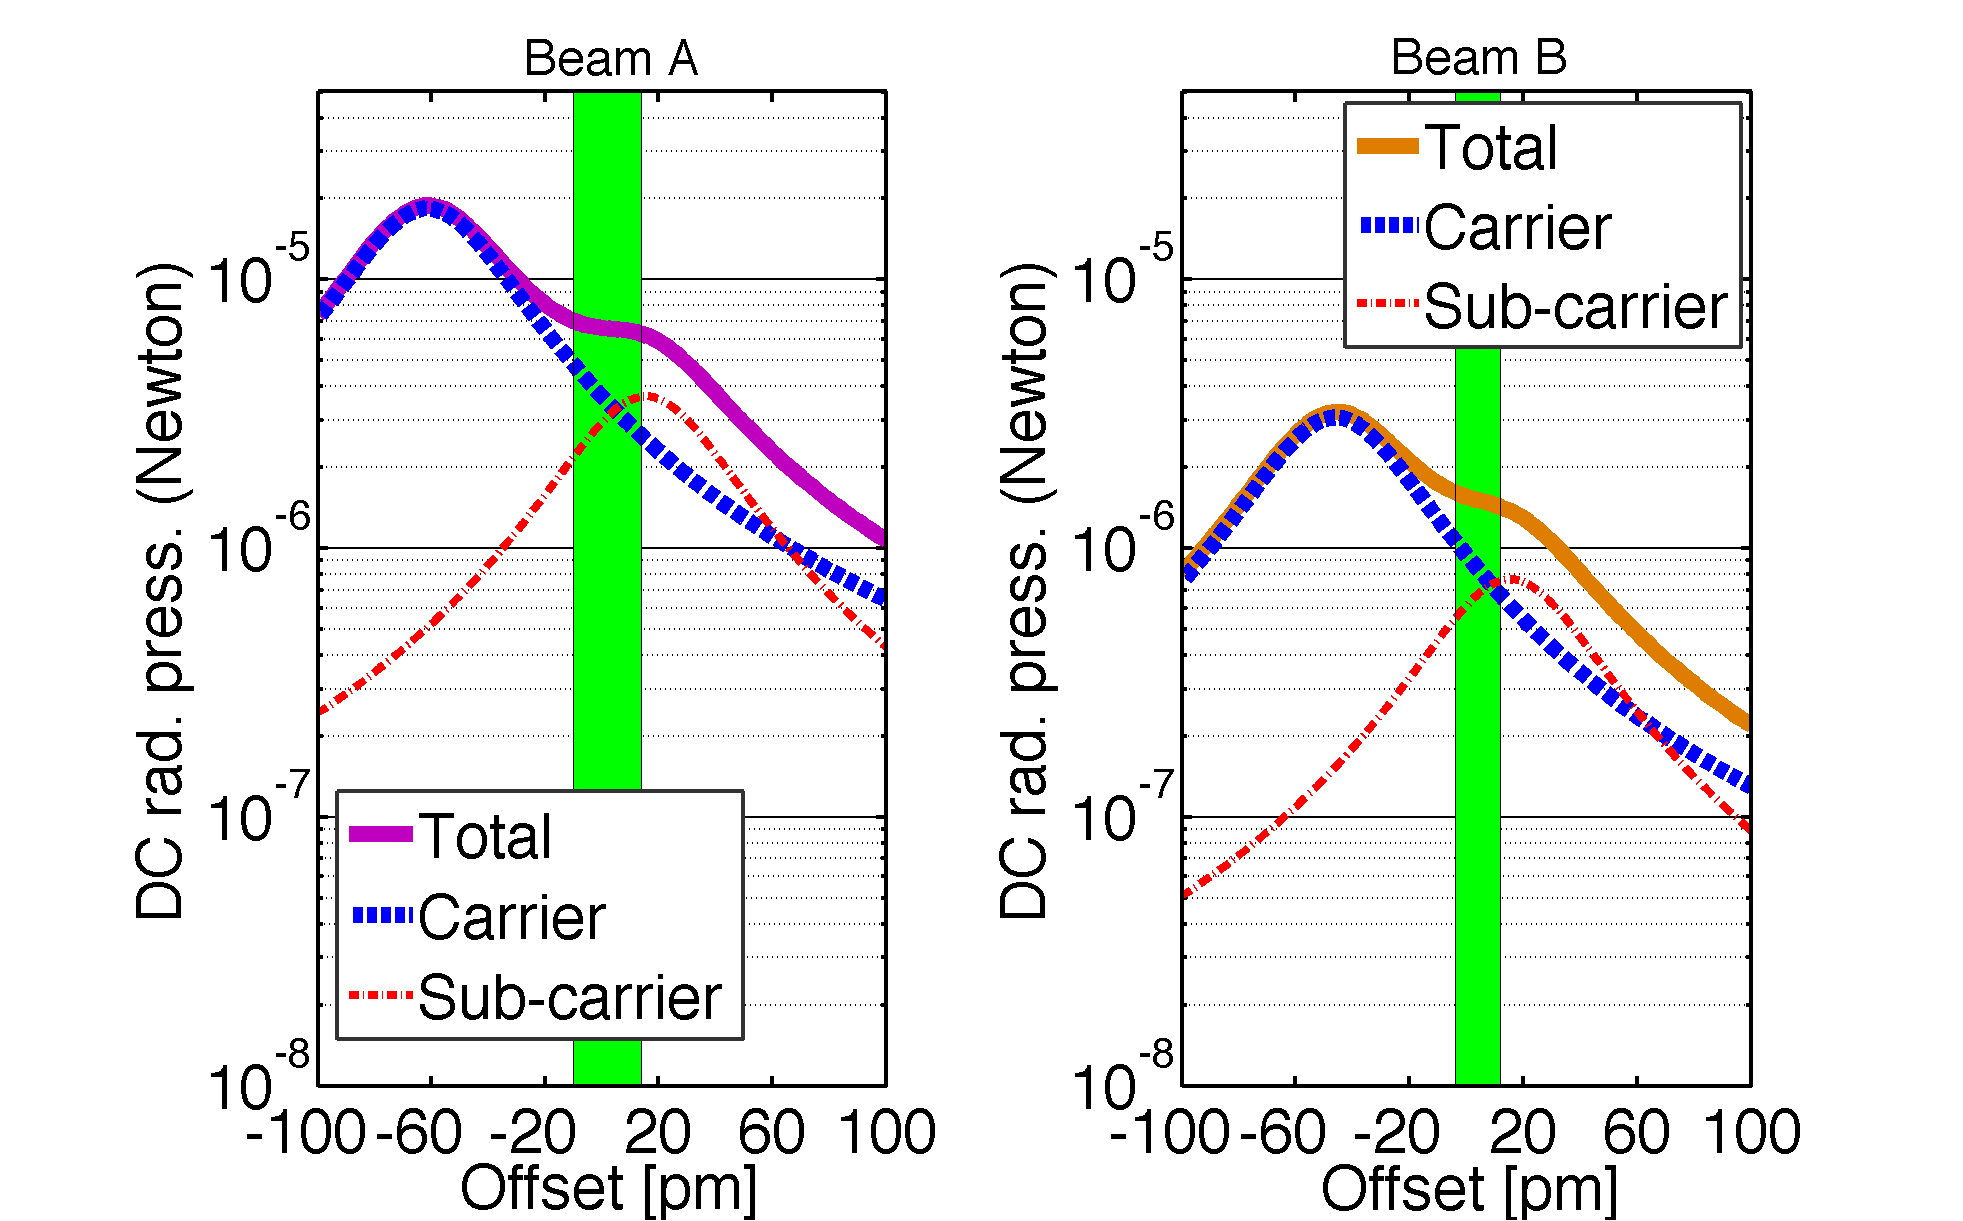
\includegraphics[width=15cm]{./figures/DC_offset_paper3.pdf}
	\caption{{Static carrier and sub-carrier build-up (calibrated in radiation pressure force) as a function of the respective cavity position. Also shown in blue is the total radiation pressure force. Using the stability testing method from section \ref{sec:stability} we find that the trap is both statically and dynamically stable in the green shaded area.
	%In Figure 4 the static (DC) radiation pressure force due to each of the four laser fields is plotted 
%as a function of cavity position. Indicated by green shading are the regions with a stable optical 
%spring (statically and dynamically). 
With the chosen model parameters those regions are about 
20 picometers wide.}}
	\label{fig:stability_region}
\end{figure}

%\tcb{Finally, Fig...... shows a simple noise budget for this MATLAB model. It is calibrated in actual motion after the trap closed loop gain suppression. The seismic noise estimate is based on a typical ground motion filtered by a one-stage passive isolation platform with a resonance frequency of $1\,$Hz. It results in a residual RMS motion of about 1 picometer. This is smaller than the 12 picometer stability band shown in Figure 4. Therefore it should be possible to turn off any feedback to the cavity length or laser frequency. The two cavities will remain locked purely due to the radiation pressure trapping force, thus trapping the payload.}


\section{Angular instability}
\label{sec:IV} 
When operated with high intracavity laser power, suspended Fabry-Perot cavities like the arm cavities of LIGO have a well known angular instability. It  arises from coupling the misalignment of the two cavity mirrors to radiation pressure torques. This is known as the Sidles-Sigg instability \cite{Sidles06}. In this section we show that the intrinsic strength of an optical trap for alignment degrees of freedom is generally bigger, i.e. has a bigger spring constant than any associated Sidles-Sigg instability. 

We start with a cavity of length $L$, with $x_1,x_2$  being the position of the beam spots on mirrors 1 and 2. $\theta_1,\theta_2$ are the yaw angles of the two mirrors, and $R_1,R_2$ are their radii of curvature. The corresponding g-factors are $g_{1,2}=1-L/R_{1,2}$.
If one or both of the mirrors are slightly misaligned ($\theta_{1,2}\neq 0$), then the radiation pressure force exerts torques $T_1$ and $T_2$ on the two mirrors, given by the following relation (see for instance \cite{Sidles06} or \cite{Ballmer13}): 
\begin{equation}
\label{SidlesSigg_Basic}
\left(
\begin{array}{c}
T_1\\
T_2
\end{array}
\right)
=
\frac{F_0 L}{1-g_1 g_2}
\left(
\begin{array}{cc}
g_2 & -1\\
-1 & g_1
\end{array}
\right)
\left(
\begin{array}{c}
\theta_1\\
\theta_2
\end{array}
\right)
\end{equation} 
with $F_0=P_0\frac{t_1^2}{(1-X)(1-\overline{X})} \frac{2 r_2^2}{c}$ being the intra-cavity radiation pressure force. Sidles and Sigg first pointed out that, since the determinant of the matrix in this equation
%\ref{SidlesSigg_Basic}
 is negative, the two eigenvalues have opposite sign. This always leads to one stable and one unstable coupled alignment degree of freedom.

First we note that for a situation in which one mass is sufficiently heavy that we can neglect any radiation pressure effects on it (i.e. $\theta_1=0$), it is sufficient to choose a negative branch cavity (i.e. $g_1<0$ and $g_2<0$) to stabilize the setup. This is for instance the case for the example setup described in Fig. \ref{fig:angular}.

Next we want to compare the order of magnitude of this effect to the strength of an angular optical spring. If we call $h$ the typical distance of the beam spot from the center of gravity of the mirror, and $x$ the cavity length change at that spot, the order of magnitude of the optical spring torque is:
\begin{eqnarray}
%F=K_{0}\cdot x = T/h\approx \frac{F_0L}{h}\cdot \frac{x}{h}
T\approx \frac{F_0 L}{1-g_1g_2}\cdot \frac{x}{h}
\end{eqnarray}
We can express this as the strength of an optical spring located at position $h$. The corresponding spring constant $K_{SS} \approx T/(h x)$. Thus we can see that
\begin{eqnarray}
\label{eqn:KSS_def}
K_{SS} \approx \frac{F_0}{1-g_1g_2}\cdot \frac{L}{h^2}.
\end{eqnarray}
We now consider the adiabatic optical spring ($\Omega=0$) in equation \ref{eqn:K0}.  Expressed in terms of $F_0$, $K_{OS}$ becomes
\begin{eqnarray}
\label{eqn:KOS_exact}
K_{OS}=i F_0 \frac{X-\overline{X}}{(1-X)(1-\overline{X})}   2 k
\end{eqnarray}
Since we operate near the maxium of the optical spring, the order of magnitude of the resonance term can be estimated as
\begin{eqnarray}
\label{eqn:res_est}
\frac{X-\overline{X}}{(1-X)(1-\overline{X})} \approx \frac{-i}{1-|X|}
\end{eqnarray}
Thus we can estimate the magnitude of  $K_{OS}$ as
\begin{eqnarray}
\label{eqn:K0_order}
K_{OS} \approx F_0 \frac{4\pi}{\lambda}\frac{1}{1-|X|} \approx F_0 \frac{4}{\lambda} \mathcal{F}
\end{eqnarray}
where $\mathcal{F}$ is the cavity finesse.
From equations \ref{eqn:KSS_def} and \ref{eqn:K0_order} we see that the optical spring $K_{OS}$  is much larger than the Sidles-Sigg instability spring $K_{SS}$ if
\begin{eqnarray}
\label{eqn:h2}
h^2 >> \frac{\lambda L}{\pi} \frac{1}{1-g_1 g_2} \frac{\pi}{4 \mathcal{F}}
\end{eqnarray}
Now recall that the beam spot size in a Fabry-Perot cavity is given by \cite{Siegman86}
\begin{equation}
w_1^2 = \frac{\lambda L}{\pi} \sqrt{\frac{g_2}{g_1(1-g_1 g_2)}}
\label{equ:spotsize1}
\end{equation} 
Assuming a symmetric cavity ($g_1=g_2$) for simplicity, we thus find that $K_{OS}$  dominates over $K_{SS}$ if
\begin{eqnarray}
\label{eqn:h2w}
h^2 >> w_{1,2}^2 \frac{1}{\sqrt{1-g_1 g_2}} \frac{\pi}{4 \mathcal{F}}
\end{eqnarray}
This condition is naturally fulfilled since we need to operate the angular optical spring with separate beams ($h>w_{1,2}$) and a large finesse ($\mathcal{F}>>1$). Therefore the angular optical spring is indeed strong enough to stabilize the Sidles-Sigg instability.

\section{Radiation Pressure Noise}
\label{sec:V}
Another advantage of radiation pressure control, compared to a classical approach based on photo detection and feedback, is its fundamental noise limit. Unlike in the classical approach, the shot noise and other sensing noises %from detecting a potentially small sample of the beam 
never enter a radiation-pressure-based feedback loop. Even though technical laser noise is typically bigger in the simple cavity setup discussed in this paper, the only fundamental noise source of the scheme is quantum radiation pressure noise. In this section we give the full expression for radiation pressure noise in the case of a dual-carrier stable optical spring.

First, we note that as long as we are interested in frequencies much smaller than the any of the features in the detuned cavity transfer function, the radiation pressure noise is relatively simple. If we also assume that the end mirror has a reflectivity of 1, the one-sided ($f\ge0$) radiation-force amplitude spectral noise density is given by
\begin{eqnarray}
\label{eqn:simpleRPN}
S_F (f) = \frac{2}{c} G \sqrt{2 \hbar \omega P_{\rm in}}
\end{eqnarray}
where $G$ is the power gain of the cavity in the detuned configuration, and $P_{\rm in}$ is the power of the shot noise limited beam entering the cavity.
Equation \ref{eqn:simpleRPN} is valid for carrier and subcarrier separately.
Note that this equation does not hold if the end mirror has a finite transmissivity, as quantum fluctuations entering from that port will also contribute to the intra-cavity shot noise. In the case of a critically coupled cavity, this will result in an increase of the intra-cavity radiation-force amplitude spectral noise density by exactly a factor of 2.

To calculate the exact expression for the radiation pressure noise induced cavity fluctuations, we first realize that we can calculate the radiation-force amplitude spectral noise for a static cavity, and then compute the response of the dual-carrier optical spring system to that driving force. This yields the correct answer up to first order in the size of the quantum fluctuations. For the calculation we track the quantum vacuum fluctuations entering at both ports of the cavity. It is useful to introduce a function $F$:
\begin{eqnarray}
\label{eqn:RPNfunction}
F(f) = F\left(\frac{\Omega + \delta + \omega_{res}}{2 \pi}\right) =& \frac{1}{1-XY^2}  \\ =& \frac{1}{1-r_1r_2e^{-2 i \delta\tau}e^{-2 i \Omega\tau}}
\end{eqnarray}
The amplitude build-up factors for fluctuations at frequency $f$ entering through the input coupler (1) and the end mirror (2) thus are
\begin{eqnarray}
\label{eqn:RPNfunction12}
 t_1 F(f) \,\,\, {\rm and} \,\,\ r_1 t_2 F(f), 
\end{eqnarray}
where we already dropped the one-way propagation factor because it drops out in the radiation force noise calculation below. 
We can now introduce the notation $F_0=F(f_0)$, $F_+=F(f_0+f)$ and $F_-=F(f_0-f)$. We then get the following expression for the one-sided radiation-force power spectral density for either carrier or sub-carrier.
\begin{eqnarray}
\label{eqn:RPN_P}
S_F (f) = \frac{2}{c} S_P (f) \,\,\,\,\,\, {\rm and}
\end{eqnarray}
\begin{eqnarray}
\label{eqn:RPN}
|S_P (f)|^2 =   \hbar \omega P_0 t_1^2|F_0|^2 (t_1^2 \!\!+\! r_1^2t_2^2)( |F_+|^2 \!\!+\!  |F_-|^2)
\end{eqnarray}
Here $P_0$ is the entering carrier power, and $f_0$ is its frequency. We can see that we recover equation \ref{eqn:simpleRPN} in the limit $t_2 \rightarrow 0$ and $G/t_1^2=|F_0|^2=|F_+|^2=|F_-|^2$. The resulting force noise from carrier and sub-carrier for the cavity A in the example above is plotted in Fig.\ref{fig:RFASD} (\emph{top}).
\begin{figure}[htbp]
	\centering
		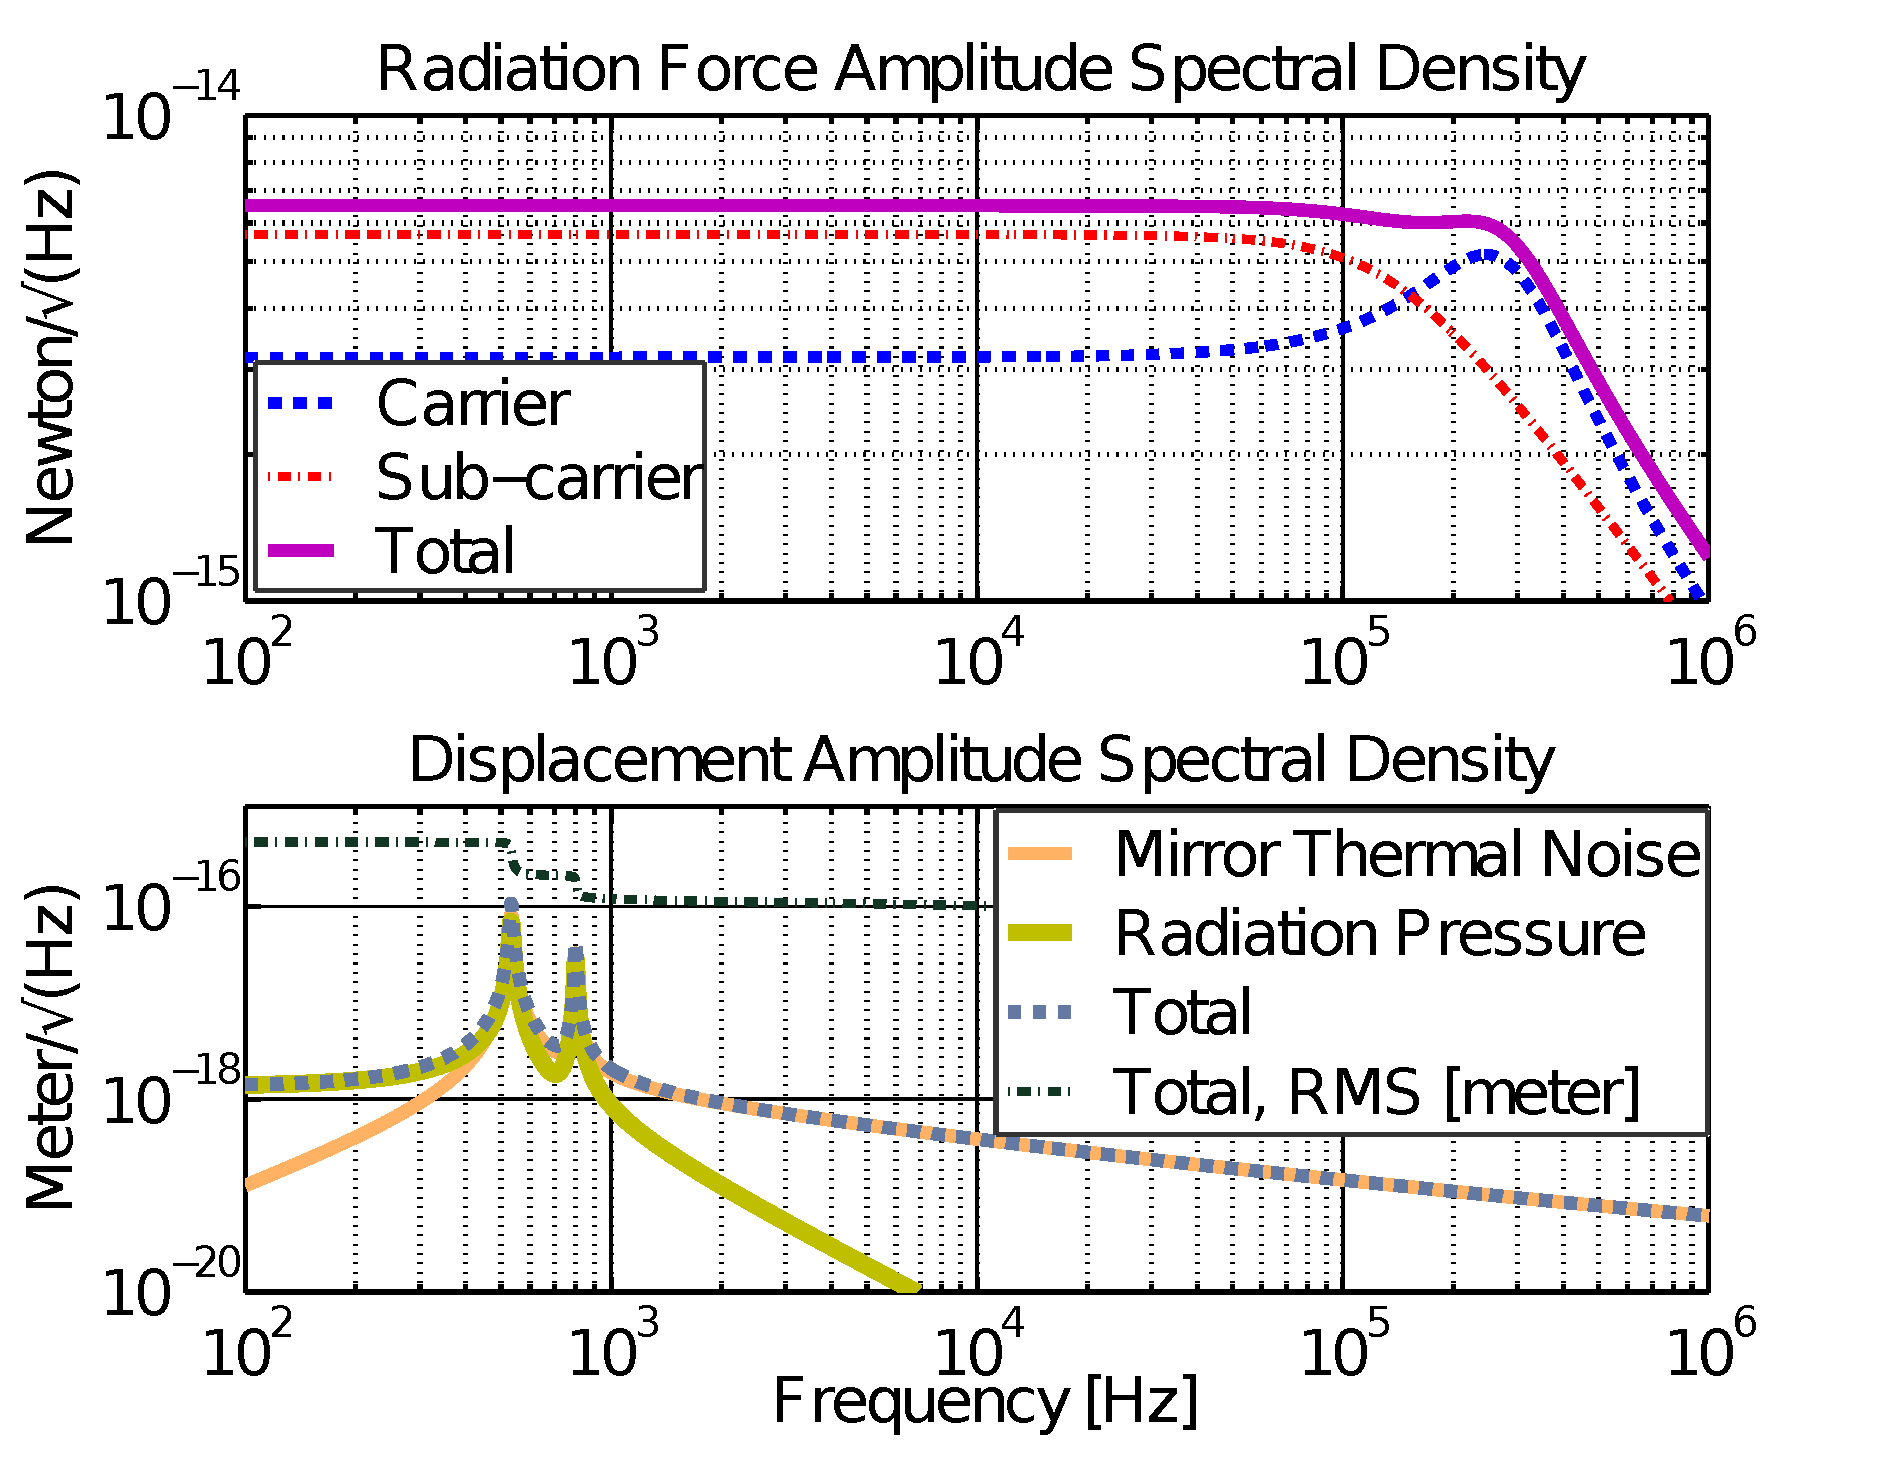
\includegraphics[width=15cm]{./figures/trap_radPresA_paper2.pdf}
	\caption{(\emph{Top}) Radiation force amplitude spectral density for the dual-carrier optical spring used in beam A of the above example. The sub-carrier dominates the noise at low frequency, but the higher-power carrier contributes more at high frequencies. Also note that if we choose the same free spectral range for the two carriers, there would be an additional beat note at the difference frequency of $310~{\rm kHz}$. (\emph{Bottom})  Radiation pressure and thermal noise displacement amplitude spectral density. The radiation pressure noise is calculated using the opto-mechanical response given in equation \ref{eqn:closedloop_tf}. The thermal noise is based on a theoretical calculation described in \cite{Saulson90}, \cite{Ballmer13}. Since seismic and suspension thermal noise depend on the experimental implementation, they are not shown, but they would also be suppressed by the optical spring closed loop response. The residual RMS motion due to the shown noise sources is less than $10^{-3}$ picometer. With the total RMS motion smaller than the 20 picometer stability band shown in Fig.\ref{fig:stability_region}, the two cavities will remain locked purely due to the radiation pressure trapping force.}
	\label{fig:RFASD}
\end{figure}

Next we calculate the response of the coupled opto-mechanical system to this driving force, using the following closed loop transfer function obtained from equations \ref{eq:MF} and \ref{eq:HX}:

\begin{eqnarray}
\label{eqn:closedloop_tf}
x = {M}({1-HM})^{-1}F
\end{eqnarray}

Above the optical spring resonances this leads to a $1/f^2$ fall-off of the displacement noise, as expected for radiation pressure noise. Meanwhile below the resonance, due to the closed loop suppression, we will have a flat displacement noise. %at a level of $S_x(f) ~ S_F(f)/K_{OS}$. 
Fig.\ref{fig:RFASD} bottom illustrates this in the case of the two-dimensional angular trap discussed above.

Finally we compare the resulting displacement noise to a classical photo-detection feedback control scheme with similar control bandwidth and control loop shape. If such a system is able to detect all availabe power and has no other dominating sensing noise sources, it can at best achieve a shot noise sensitivity of 
\begin{eqnarray}
\label{eqn:classyShot}
S_x \backsim \frac{l}{P_0}\sqrt{2 \hbar \omega P_0}
\end{eqnarray}
where $l$ is the cavity line width in meters. To have the same control bandwidth and loop shape the system needs a controller transfer function equal to the optical spring, $H = K_{OS} \backsim \frac{2 G P_0}{c l}$, and hence it will have a  noise performance similar to equation \ref{eqn:simpleRPN},  $H S_x=S_F$.  
Thus we find that the traditional control scheme can only achieve similar noise if all the power from the cavity is detected, and there are no other relevant sensing noise sources. 

%\section{TBD...NOISE?}
%Here I put some calculation made together with Stefan...(no text yet)
%\begin{eqnarray}
%E_{tot}=E_{0}^{tot} \left [1 + \alpha_+ e^{i\Omega t} E_+^{tot} +  \alpha_-^* e^{-i\Omega t} E_-^{tot}  \right ]
%\end{eqnarray}
%with
%\begin{eqnarray}
%\alpha^+= \frac{(a + i\phi)}{2}  \quad \mbox{and} \quad  \alpha^-= \frac{(a - i\phi)}{2}
%\end{eqnarray}
%where $a$ and $\phi$ are both complex numbers (is that necessary????).
%Recalling that:
%\begin{eqnarray}
%E_0^{tot}=t \frac{E}{1-X}, 
%X=r_1r_2e^{-ikL}, \\
%X_\pm=r_1r_2e^{-1K_\pm L}
%\end{eqnarray}
%we have
%\begin{eqnarray}
%E_{tot}=\frac{E_0t}{1-X}\left [ 1 +  \alpha_+' e^{i\Omega t}  +\alpha_-^{'*} e^{-i\Omega t}  \right ]
%\end{eqnarray}
%with
%\begin{eqnarray}
%\alpha_+' =  \frac{1-X}{1-X_+}\alpha_+ \quad \mbox{and} \quad \alpha_-^{'*} = \frac{1-X}{1-X_-} \alpha_-^* 
%\end{eqnarray}



\section{Conclusions}
In conclusion, we investigated the use of the radiation pressure of the laser light as an alternative to a conventional feedback system for controlling the 
longitudinal and angular degree of freedom of a mirror.
The method is based on a double dual-carrier scheme, using a total of four detuned laser fields in two cavities. 
The two dual-carrier beams hit the mirror in separate spots, forming two stable optical springs.
%Each dual-carrier beam hits the test mirror in two different spots, trapping the mirror in these two points. 
This constrains both the longitudinal and the angular degrees of freedom of the mirror, replacing completely the commonly used electronic feed-back system.
%We propose a system with two longitudinal traps acting on different spots of a single mirror; together, these traps will constrain both the position and one angular degrees of freedom of the mirror. This essentially replaces the magnetic drives with optical traps. The idea is promising and will be easy to apply to additional angular degree of freedom as well.
We showed that this setup allows a stable control of the two degrees of freedom, within a displacement range of the test mirror of $\sim 20\,$pm. This promising idea can be extended to the other angular degree of freedom.
We found that such a method creates an angular optical spring stronger than the angular Sidles-Sigg instability, which drives the requirement for angular control in the high power arm cavities of gravitational wave detectors. We also showed that the fundamental limit of this scheme is the quantum radiation pressure noise, resulting in a reduction in control noise compared to a conventional active feedback approach. 
%\tcr{This is a promising idea easily to extend to other degrees of freedom.}
We are working towards the experimental demonstration of this effect for a gram-scale mirror and beginning to explore its extension
to large-scale gravitational wave detectors.
%\tcb{Shall we talk about FIG.\ref{fig:stability_region}}


%Inline math may be typeset using the \verb+$+ delimiters. Bold math
%symbols may be achieved using the \verb+bm+ package and the
%\verb+\bm{#1}+ command it supplies. For instance, a bold $\alpha$ can
%be typeset as \verb+$\bm{\alpha}$+ giving $\bm{\alpha}$. Fraktur and
%Blackboard (or open face or double struck) characters should be
%typeset using the \verb+\mathfrak{#1}+ and \verb+\mathbb{#1}+ commands
%respectively. Both are supplied by the \texttt{amssymb} package. For
%example, \verb+$\mathbb{R}$+ gives $\mathbb{R}$ and
%\verb+$\mathfrak{G}$+ gives $\mathfrak{G}$
%
%In \LaTeX\ there are many different ways to display equations, and a
%few preferred ways are noted below. Displayed math will center by
%default. Use the class option \verb+fleqn+ to flush equations left.
%
%Below we have numbered single-line equations; this is the most common
%type of equation in \textit{Physical Review}:
%\begin{eqnarray}
%\chi_+(p)\alt{\bf [}2|{\bf p}|(|{\bf p}|+p_z){\bf ]}^{-1/2}
%\left(
%\begin{array}{c}
%|{\bf p}|+p_z\\
%px+ip_y
%\end{array}\right)\;,
%\\
%\left\{%
% \openone234567890abc123\alpha\beta\gamma\delta1234556\alpha\beta
% \frac{1\sum^{a}_{b}}{A^2}%
%\right\}%
%\label{eq:one}.
%\end{eqnarray}
%Note the open one in Eq.~(\ref{eq:one}).
%
%Not all numbered equations will fit within a narrow column this
%way. The equation number will move down automatically if it cannot fit
%on the same line with a one-line equation:
%\begin{equation}
%\left\{
% ab12345678abc123456abcdef\alpha\beta\gamma\delta1234556\alpha\beta
% \frac{1\sum^{a}_{b}}{A^2}%
%\right\}.
%\end{equation}
%
%When the \verb+\label{#1}+ command is used [cf. input for
%Eq.~(\ref{eq:one})], the equation can be referred to in text without
%knowing the equation number that \TeX\ will assign to it. Just
%use \verb+\ref{#1}+, where \verb+#1+ is the same name that used in
%the \verb+\label{#1}+ command.
%
%Unnumbered single-line equations can be typeset
%using the \verb+\[+, \verb+\]+ format:
%\[g^+g^+ \rightarrow g^+g^+g^+g^+ \dots ~,~~q^+q^+\rightarrow
%q^+g^+g^+ \dots ~. \]
%
%
%\subsection{Multiline equations}
%
%Multiline equations are obtained by using the \verb+eqnarray+
%environment.  Use the \verb+\nonumber+ command at the end of each line
%to avoid assigning a number:
%\begin{eqnarray}
%{\cal M}=&&ig_Z^2(4E_1E_2)^{1/2}(l_i^2)^{-1}
%\delta_{\sigma_1,-\sigma_2}
%(g_{\sigma_2}^e)^2\chi_{-\sigma_2}(p_2)\nonumber\\
%&&\times
%[\epsilon_jl_i\epsilon_i]_{\sigma_1}\chi_{\sigma_1}(p_1),
%\end{eqnarray}
%\begin{eqnarray}
%\sum \vert M^{\text{viol}}_g \vert ^2&=&g^{2n-4}_S(Q^2)~N^{n-2}
%        (N^2-1)\nonumber \\
% & &\times \left( \sum_{i<j}\right)
%  \sum_{\text{perm}}
% \frac{1}{S_{12}}
% \frac{1}{S_{12}}
% \sum_\tau c^f_\tau~.
%\end{eqnarray}
%\textbf{Note:} Do not use \verb+\label{#1}+ on a line of a multiline
%equation if \verb+\nonumber+ is also used on that line. Incorrect
%cross-referencing will result. Notice the use \verb+\text{#1}+ for
%using a Roman font within a math environment.
%
%To set a multiline equation without \emph{any} equation
%numbers, use the \verb+\begin{eqnarray*}+,
%\verb+\end{eqnarray*}+ format:
%\begin{eqnarray*}
%\sum \vert M^{\text{viol}}_g \vert ^2&=&g^{2n-4}_S(Q^2)~N^{n-2}
%        (N^2-1)\\
% & &\times \left( \sum_{i<j}\right)
% \left(
%  \sum_{\text{perm}}\frac{1}{S_{12}S_{23}S_{n1}}
% \right)
% \frac{1}{S_{12}}~.
%\end{eqnarray*}
%
%To obtain numbers not normally produced by the automatic numbering,
%use the \verb+\tag{#1}+ command, where \verb+#1+ is the desired
%equation number. For example, to get an equation number of
%(\ref{eq:mynum}),
%\begin{equation}
%g^+g^+ \rightarrow g^+g^+g^+g^+ \dots ~,~~q^+q^+\rightarrow
%q^+g^+g^+ \dots ~. \tag{2.6$'$}\label{eq:mynum}
%\end{equation}
%
%\paragraph{A few notes on \texttt{tag}s} 
%\verb+\tag{#1}+ requires the \texttt{amsmath} package. 
%Place the \verb+\tag{#1}+ command before the \verb+\label{#1}+, if any. 
%The numbering produced by \verb+\tag{#1}+ \textit{does not affect} 
%the automatic numbering in REV\TeX; 
%therefore, the number must be known ahead of time, 
%and it must be manually adjusted if other equations are added. 
%\verb+\tag{#1}+ works with both single-line and multiline equations. 
%\verb+\tag{#1}+ should only be used in exceptional cases---%
%do not use it to number many equations in your paper. 
%Please note that this feature of the \texttt{amsmath} package
%is \emph{not} compatible with the \texttt{hyperref} (6.77u) package.
%
%Enclosing display math within




%\begin{acknowledgments}
%We would like to thank Peter Saulson, Prayush Kumar, Riccardo Penco and Matt West for the many fruitful discussions. This work was supported by the National Science Foundation grant PHY-1068809. This document has been assigned the LIGO Laboratory document number  LIGO-P1300224.
%\end{acknowledgments}

%\appendix
%\section{Optical spring constant derivation}
\label{app:A} 
%\subsection{Optical spring constant}
%\label{sec:Apx1}

In this section we consider the effect of light stored in a detuned Fabry-Perot cavity using a classical approach.
The intra-cavity power generates radiation pressure that exerts on the cavity mirror a force $F_{rad}=-K_{OS}\cdot x$,
where $x$ is the mirror displacement and $K_{OS}$ is the optical spring constant.
Here we show the full derivation of the optical spring constant $K_{OS}$.

We consider a suspended Fabry-Perot cavity of length $L_0$ %shined by a laser light 
with an incident beam of wavelength $\lambda$ and power $P_0$.
First we calculate a general expression of the intra-cavity power and then its  radiation pressure force exerted on the end mirror.\\


\begin{figure}[htbp]
	\centering
		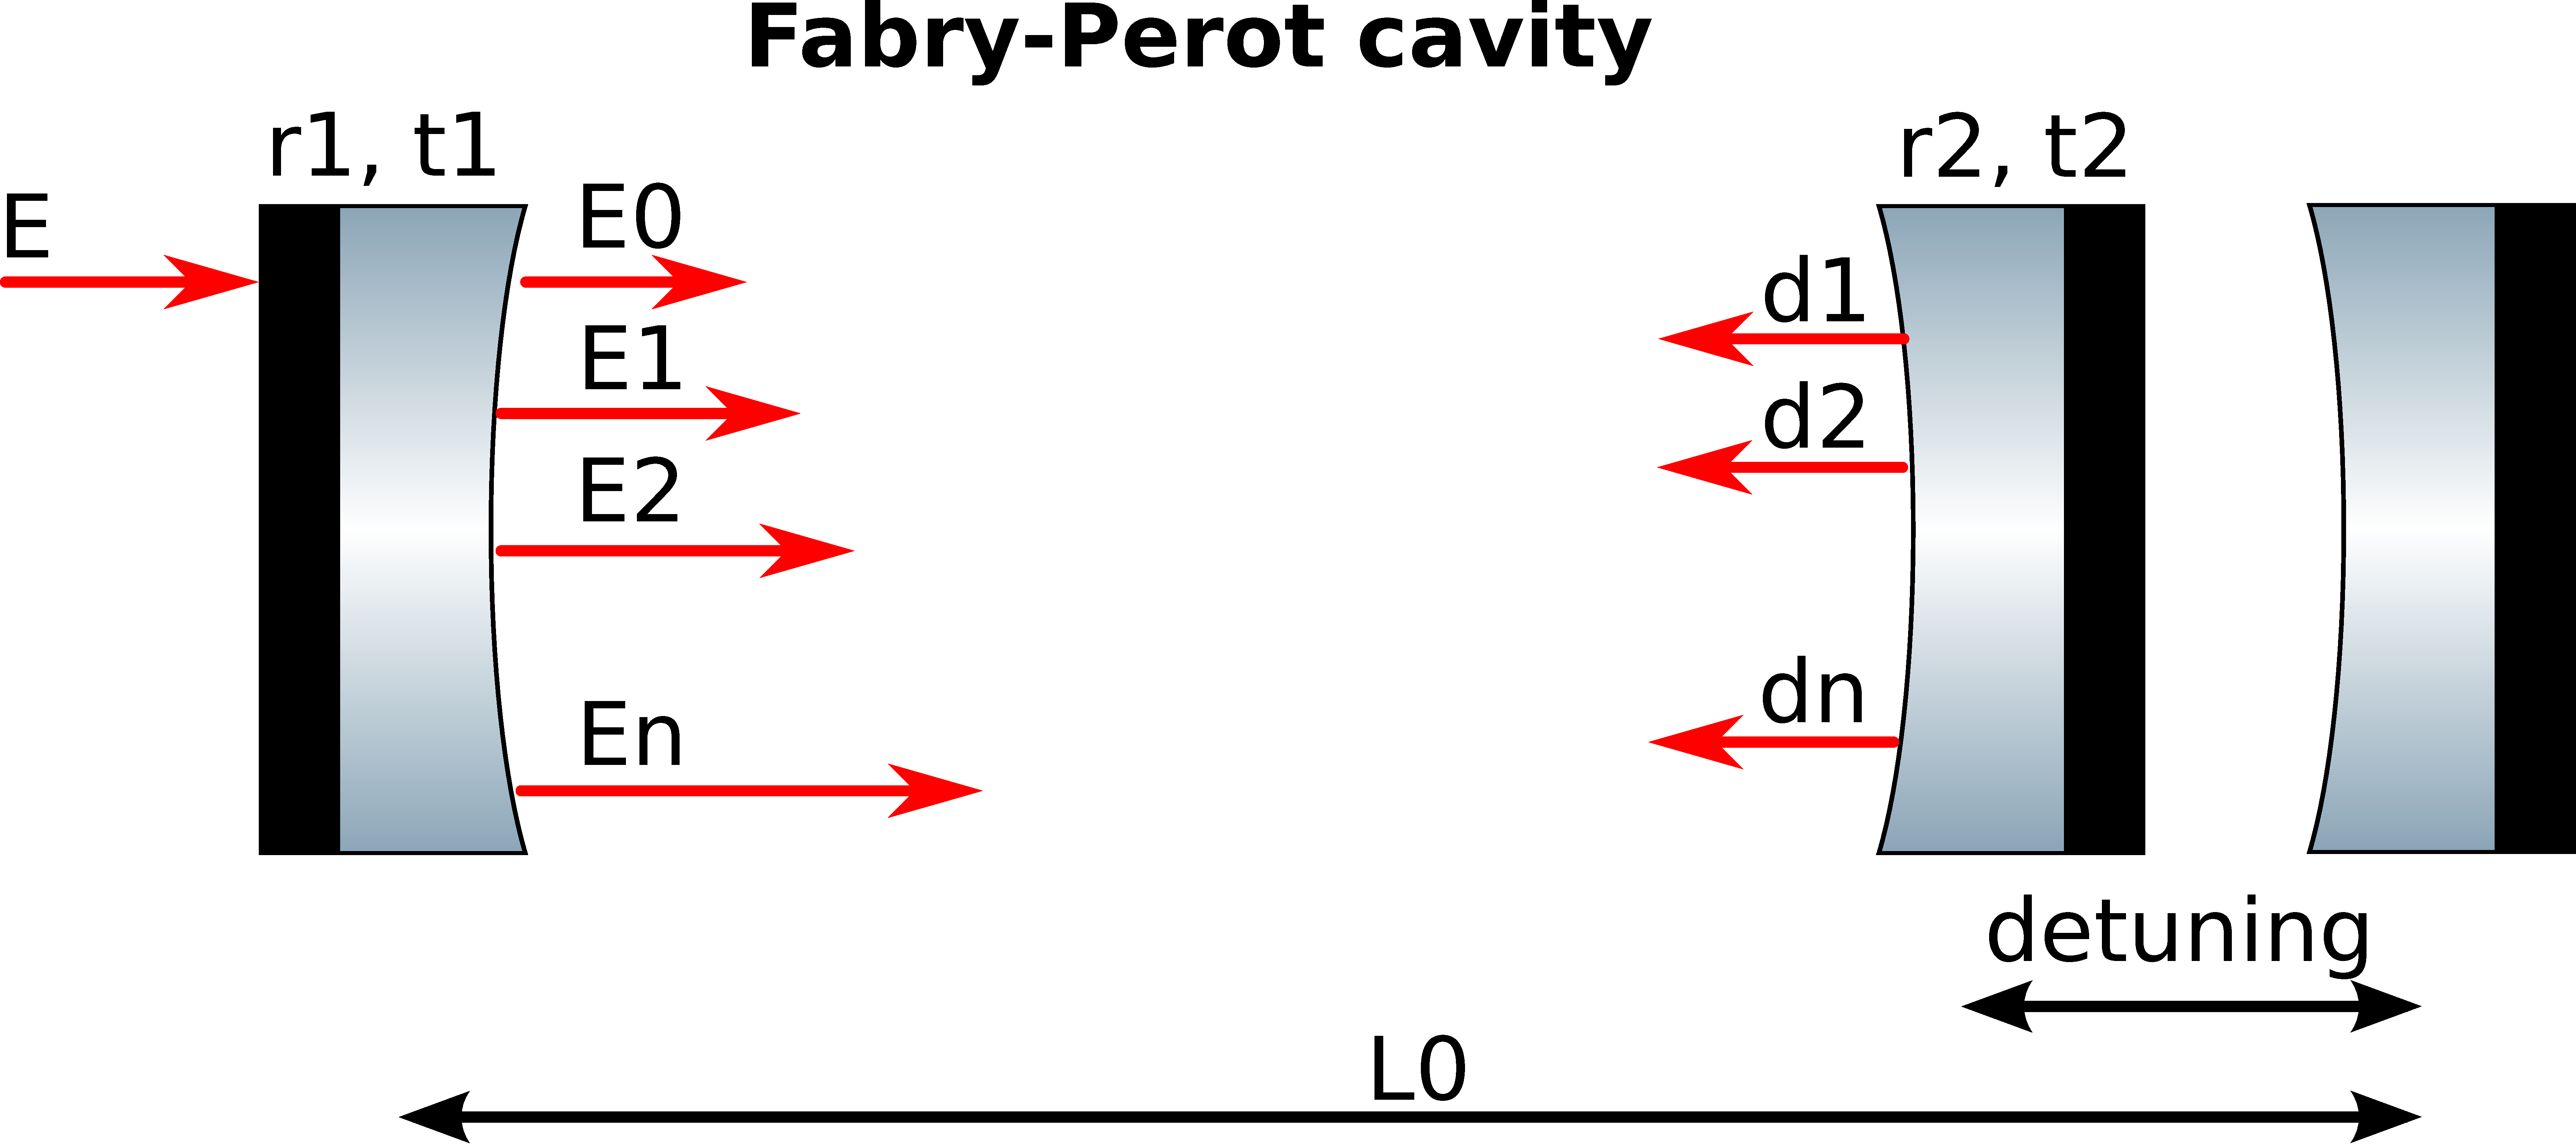
\includegraphics[width=8cm]{./images/cavity_paper.pdf}
	\caption{A Fabry-Perot cavity of length $L_0$ and coefficients $r_1,t_1$ and $r_2,t_2$ for the input and end mirrors respectively. 
	The input mirror is stationary while the end mirror is affected by harmonic motion. The incoming field $E$ at each round-trip $i$ adds up a phase shift due to the displacement $d_i$}
	\label{fig:cavity_k}
\end{figure}


The field $E=A_0e^{i\omega t}$ enters the cavity through the input mirror of coefficient $t_1=t$ and $r_1$ and the field inside the cavity at the input mirror can be seen as following

\begin{eqnarray}
E_{tot}=E_0+E_1+E_2+E_3+...+En+...
\end{eqnarray}


We consider in our model the following definitions, with $d_n$ being the displacement of the mirror,

\begin{eqnarray}
L_1&=&2(L_0+d_1)\\
L_2&=&2(2L_0+d_1+d_2)\nonumber\\
L_3&=&2(3L_0+d_1+d_2+d_3)\,\, \nonumber\\ %\mbox{with} \,\,d_n=d(t-(2n-1)\tau)\nonumber\\
...\nonumber
\end{eqnarray}
with 
\begin{eqnarray}
\label{eqn:dn1}
d_n &=& d(t-[(2n-1)\tau + \alpha_n ]) \quad \mbox{and}\\
\label{eqn:dn2}
\alpha_n &=& 2\sum\limits_{l=1}^{n-1}\frac{d_l}{c}-\frac{d_n}{c}
\end{eqnarray}

where $\tau=L_0/c$.
With the round trip length $L=2L_0$  we obtain

\begin{eqnarray}
E_{tot}&=&tE(1\!+\!r_1r_2 e^{-ikL_1}\!\!+\!(r_1r_2)^2 e^{-ikL_2}\nonumber\\
&+&(r_1r_2)^3 e^{-ikL_3}  \cdots )\nonumber\\
&=&tE(1\!+\!r_1r_2 e^{-ikL}e^{-2ikd_1}\!\!+\!(r_1r_2)^2 e^{-2ikL}e^{-2ik(d_1\!+\!d_2)}\nonumber\\
&+&(r_1r_2)^3 e^{-3ikL}e^{-2ik(d_1\!+\!d_2\!+\!d_3)}  \cdots )\nonumber
\end{eqnarray}



If we define $X=r_1r_2 e^{-ikL}$ we have 

\begin{eqnarray}
E_{tot}=tE(1+Xe^{-2ikd_1} +X^2e^{-2ik(d_1+d_2)}\nonumber\\
+X^3e^{-2ik(d_1+d_2+d_3)} \cdots )\nonumber
\end{eqnarray}

Since by definition the optical spring $K_{OS}$ is the linear term in the expansion $F=F_0+ K_{OS} d + O(d^2)$, we now expand the exponential in $d_n$. We group  $d_n$ terms:

\begin{eqnarray}
E_{tot}&=&tE(1+X(1-2ikd_1) +X^2(1-2ik(d_1+d_2))\nonumber\\
&+&X^3(1-2ik(d_1+d_2+d_3)) + \cdots )\nonumber \\
\nonumber \\
&=&tE(1+X+X^2+X^3 +\cdots\nonumber\\
&-& 2ikd_1(X+X^2+X^3\cdots)\nonumber\\
&-&2ikd_2(X^2+X^3+X^4\cdots)\nonumber\\  
&-&2ikd_3(X^3+X^4+X^5\cdots)+\cdots) \nonumber \\
\nonumber \\
%&=&tE(\frac{1}{1-X}-2ikd_1\frac{X}{1-X}-2ikd_2\frac{X^2}{1-X}\nonumber \\
%&-&2ikd_3\frac{X^3}{1-X}+\cdots) \nonumber \\
%\nonumber \\
&=&\frac{tE}{1-X}(1-2ikd_1 X-2ikd_2 X^2-2ikd_3 X^3+\cdots) \nonumber
\end{eqnarray}
Since any correction from $\alpha_n$ (equation \ref{eqn:dn2}) is quadratic in $d(t)$, we can again neglect it by definition, and find for the harmonic mirror motion (i.e. in the Fourier domain)
\begin{eqnarray}
d_n&=&x_0e^{i\Omega(t-(2n-1)\tau)}=x_0e^{i\Omega t}e^{-i\Omega(2n-1)\tau}\nonumber\\
&=&x_0e^{i\Omega t} \frac{Y^{2n}}{Y}\frac{Y}{Y}=Y^{2n-2}d_1
\end{eqnarray}

where $Y=e^{-i\Omega\tau}$. Thus we can write


\begin{eqnarray}
E_{tot}&=&\frac{tE}{1-X}(1-2ikd_1 X-2ikd_1 Y^2X^2\nonumber\\
&-&2ikd_1 Y^4 X^3-2ikd_1 Y^6 X^4\cdots)\\
&=&\frac{tE}{1-X}\nonumber\\
&\times &\left[1-2ikd_1 X(1+ Y^2X+ Y^4 X^2+Y^6 X^3\cdots)\right]\nonumber\\
&=&\frac{tE}{1-X}\left [1-\frac{2ikd_1 X}{1-Y^2X}\right ]
\end{eqnarray}

where $d_1$ is a complex number. Since we have to take its real part $Re (d_k)=\frac{d_k+\bar{d}_k}{2}$,
we consider the field inside the cavity with $\bar{d}_k$ conjugate of $d_k$:

\begin{eqnarray}
\frac{tE}{1-X}\left [1-\frac{2ik\bar{d}_1 X}{1-\overline{Y}^2 X}\right ]
\end{eqnarray}

and we obtain as total field $E$

\begin{eqnarray*}
E_{tot}=tE\left [\frac{1}{1-X}- \frac{2ikX}{2(1-X)}   \left ( \frac{d_1}{1-Y^2 X} +\frac{\bar{d}_1}{1-\overline{Y}^2 X}\right )\right]
\end{eqnarray*}

and its complex conjugate 

\begin{eqnarray*}
\overline{E}_{tot}=t\overline{E}\left [\frac{1}{1-\overline{X}}+\frac{2ik\overline{X}}{2(1-\overline{X})}   \left ( \frac{\bar{d}_1}{1-\overline{Y}^2 \overline{X}}+\frac{d_1}{1-Y^2 \overline{X}}\right )\right]
\end{eqnarray*}
 
Using the following expression
 
\begin{eqnarray}
d_1=x_0e^{i\Omega(t-\tau)}=x_0e^{i\Omega t}e^{-i\Omega\tau}=xY  
\end{eqnarray}
 
%Since we are interested only in the linear terms of $d_n$, 
%we neglect $O(d^2)$ terms (\tcb{Stefan could you write a sentence here to say "WHY"?})
we can now obtain the intra-cavity power expression by multiplying $E_{tot}$ by its conjugate
and considering only the linear terms of $x$
%(we neglect $O(d^2)$ terms \tcb{Stefan could you write a sentence here to say "WHY"?})
 
\begin{eqnarray}
P&=&E_{tot}\cdot \overline{E}_{tot}=P_0 t^2[ \frac{1}{(1-X)(1-\overline{X})}\nonumber\\  
&-&\frac{ikX xY}{(1-\overline{X})(1-X)(1-Y^2 X)} -
\frac{ikX \bar{x}\overline{Y}}{(1-\overline{X})(1-X)(1-\overline{Y}^2 X)}\nonumber \\
&+&\frac{ik\overline{X} \bar{x}\overline{Y} } {(1-\overline{X})(1-X)(1-\overline{Y}^2 \overline{X})}+ 
\frac{ik\overline{X} xY}{(1-\overline{X})(1-X)(1-Y^2 \overline{X})}]  \nonumber \\
%\frac{k^2 |X|^2}{4(1-X)(1-\overline{X})} \left( 
%\frac{|x|^2|Y|^2}{(1-Y^2 X)(1-\overline{Y}^2\overline{X})}+
%\frac{|x|^2|Y|^2}{(1-\overline{Y}^2 X)(1-Y^2\overline{X}) }+\nonumber 
%\frac{x^2 Y^2}{(1-Y^2 X)(1-Y^2\overline{X})}+
%\frac{\bar{x}^2 \bar{Y}^2}{(1-\overline{Y}^2 X)(1-\overline{Y}^2\overline{X})}
%\right) ]   
 %\right] 
\end{eqnarray}

where we have also neglected the first constant term. We now group the terms in $x$ and $\bar{x}$:

\newpage
\begin{eqnarray}
%\centering
P&=&-P_0t^2 [ \frac{ikY}{(1-\overline{X})(1-X)} \left( \frac{X}{1-Y^2 X}-\frac{\overline{X}}{1-Y^2\overline{X}} \right) x\nonumber\\
&+&\frac{ik\overline{Y}}{(1-\overline{X})(1-X)} \left( \frac{X}{1-\overline{Y}^2 X}-\frac{\overline{X}}{1-\overline{Y}^2\overline{X}} \right)\bar{x} ]=\nonumber \\
&=&-P_0t^2 [ \frac{ikY}{(1-\overline{X})(1-X)}\nonumber\\ 
&\times &\left( \frac{X}{1-Y^2 X}-\frac{\overline{X}}{1-Y^2\overline{X}} \right) x + cc ]
\end{eqnarray}

Once we have calculated the power we can obtain the radiation pressure force on the end mirror by $F_{rad}=\frac{2 r_2^2}{c}P$. Furthermore
we can also notice the similarity of the expression with the elastic force. Thus we recall that
in frequency domain and complex notation $K$ is defined by $F=-Kx$, the real form is thus

\begin{eqnarray*}
F'=Re[F]=-\frac{1}{2}(Kx+\overline{K}\bar{x})=-\frac{1}{2}(Kx+cc)
\end{eqnarray*}

Taking into account that we are calculating the radiation pressure on the end mirror, we need to consider an extra delay factor $Y$
for the calculation of the power which appears in the expression of $K$. The complex spring is then given by 

\begin{eqnarray*}
%\centering
K=\frac{2 r_2^2}{c} P_0 t^2  \frac{2ikY^2}{(1-\overline{X})(1-X)} \left( \frac{X}{1-Y^2 X}-\frac{\overline{X}}{1-Y^2\overline{X}} \right) 
\end{eqnarray*}
which can be rewritten in the form of equations \ref{KOS_full_2}
and \ref{eqn:K0}.


\subsection*{Detuning}
Given the frequency detuning is $\delta=\omega_0-\omega_{res}$ and $\Omega=\omega-\omega_0$,
where $\omega_0$ is the carrier (sub-carrier) frequency and $\omega_{res}$ is the resonant frequency, we get the following expressions:

\begin{eqnarray}
\mbox{\textit{Resonance}}\nonumber\\ 
\lambda_{res}&=& L/n, \quad k_{res}=\frac{2\pi n}{L}, \nonumber\\ 
\omega_{res} & = & k_{res}\cdot c = \frac{2\pi n}{L} \cdot c\\
\mbox{\textit{Carrier}}\nonumber\\ 
\lambda_0 & = &\lambda,  \quad k_0=\frac{2\pi}{\lambda}=k, \nonumber\\ 
\omega_0 & = & k_0\cdot c=\frac{2\pi c}{\lambda}=w_{res}+\delta\\
\mbox{\textit{Sideband}}\nonumber\\
\omega &=& \Omega+\omega_0=\Omega+\delta+\omega_{res}
\end{eqnarray}

Thus we find
\newpage
\begin{eqnarray}
e^{-ikL}\equiv e^{-ik_0L}=e^{-i\omega_0 \frac{L}{c}}\nonumber\\
=e^{-i(\omega_{res}+\delta)\frac{L}{c}}=e^{-i\omega_{res}\frac{L}{c}}e^{-i\delta\frac{L}{c}}
\end{eqnarray}
Recalling that $\tau=\frac{L_0}{c}=\frac{L}{2c}$ we can write
\begin{eqnarray}
e^{-ikL}=e^{-i\delta 2\tau}%\approx 1-i\delta 2\tau
\end{eqnarray}

%For a negative  detuning
%\begin{eqnarray}
%e^{-ikL} &=& e^{-i(\omega_{res}-\delta)\frac{L}{c}}\nonumber\\
%&=&e^{-i\omega_{res}\frac{L}{c}}e^{i\delta\frac{L}{c}}% \approx 1+i\tau2\delta
%\end{eqnarray}

If we now replace $X$ and $Y$ we obtain the exact expression for $K$:%the most general expression of $K$ that has seen so far 

\begin{eqnarray}
%\centering
K_{OS}=&-P_0 t^2 r_2^2 \frac{4ike^{-2i\Omega\tau}}{c(1-r_1\!r_2e^{i2\delta\tau})(1-r_1\!r_2e^{-i2\delta\tau})}\times\nonumber\\
 & \left( \frac{r_1\!r_2e^{-i\delta \tau}}{1\!-\!r_1\!r_2e^{-2i\Omega\tau} e^{-i2\delta\tau}}
 \!-\!\frac{r_1\!r_2e^{i2\delta\tau}}{1\!-\!r_1\!r_2e^{-2i\Omega\tau}e^{i2\delta\tau}} \right) 
\end{eqnarray}


To compare to existing literature we now expand the exponentials to linear order 
in $\Omega$ and $\delta$, 
$e^{-i\delta 2\tau}\approx 1-i\delta 2\tau$
and $e^{-i2\Omega \tau}\approx 1-i2\Omega \tau$:

\begin{eqnarray}
K =& -P_0 t^2 r_2^2 \times \nonumber\\
& \frac{4ik(1-2i\Omega\tau)r_1r_2}{c(1-r_1r_2+r_1r_2i2\delta\tau)(1-r_1r_2-r_1r_2i2\delta\tau)}\times\\
& \left[\frac{1-i2\delta\tau}{1-r_1r_2(1-2i\Omega\tau-i2\delta\tau)} -\frac{1+i2\delta\tau}{1-r_1r_2(1-2i\Omega\tau+i2\delta\tau)} \right] \nonumber 
\end{eqnarray}

%\begin{eqnarray}
%=-P_0 t^2 r_2^2 \times\nonumber \\
%\frac{4ik(1-2i\Omega\tau)r_1r_2}{c(1+\frac{r_1r_2}{1-r_1r_2}i2\delta\tau)(1-\frac{r_1r_2}{1-r_1r_2}i2\delta\tau)(1-r_1r_2)^3}\nonumber\\
%\left[\frac{1-i\tau2\delta}{1+\frac{r_1r_2}{1-r_1r_2}2i\Omega\tau+\frac{r_1r_2}{1-r_1r_2}i2\delta\tau} -
%\frac{1+i\tau2\delta}{1+\frac{r_1r_2}{1-r_1r_2}2i\Omega\tau-\frac{r_1r_2}{1-r_1r_2}i2\delta\tau}
%\right]\nonumber
%\end{eqnarray}

Considering the $Finesse \approx \pi \frac{r_1r_2}{1-r_1r_2}= \pi FSR/\gamma$, the cavity bandwidth $\gamma$, and the free spectral range $FSR=1/2\tau$, we obtain:

\begin{eqnarray}
K_{OS}\approx-P_0 t^2 r_2^2 \frac{4ik(1-2i\Omega\tau)r_1r_2}{c(1+i\frac{\delta}{\gamma})(1-i\frac{\delta}{\gamma})(1-r_1r_2)^3} \nonumber\\
\times\left[\frac{1-i2\delta}{1+\frac{\Omega}{\gamma}i+\frac{\delta}{\gamma}i} -
\frac{1+i2\delta}{1+\frac{\Omega}{\gamma}i-\frac{\delta}{\gamma}i}
\right]
\end{eqnarray}

Finally, since they correspond to a simple time delay, we neglect the $i\Omega\tau$, $i\delta\tau$ terms in the numerator and obtain
\begin{eqnarray}
K_{OS} & \approx & P_0 t^2 r_2^2 \frac{8k r_1r_2}{c(1-r_1r_2)^3}\frac{ \frac{\delta}{\gamma}}{(1+\frac{\delta^2}{\gamma^2})} 
\left[\frac{1}{1+\frac{\delta^2}{\gamma^2}-\frac{\Omega^2}{\gamma^2}+i2\frac{\Omega}{\gamma} }\right]\nonumber\\
%& = & \frac{K_0}{1+\frac{\delta^2}{\gamma^2}-\frac{\Omega^2}{\gamma^2}+i2\frac{\Omega}{\gamma}}
\end{eqnarray}

\subsubsection{Overcoupled cavity}

In the particular case of perfectly over-coupled cavity ($r_2=1$) $Finesse/\pi=2/T_1$ and $(1-r_1r_2)^2=T_1^2/2$ and the optical spring constant becomes:

\begin{eqnarray}
K_{OS} & \approx & 128 P_0  \frac{\pi}{c\lambda T_1^2}\frac{ \frac{\delta}{\gamma}}{(1+\frac{\delta^2}{\gamma^2})} 
\left[\frac{1}{1+\frac{\delta^2}{\gamma^2}-\frac{\Omega^2}{\gamma^2}+i2\frac{\Omega}{\gamma} }\right]\nonumber\\
\label{eqn:overcoupled}
%& = & \frac{K_0}{1+\frac{\delta^2}{\gamma^2}-\frac{\Omega^2}{\gamma^2}+i2\frac{\Omega}{\gamma}}
\end{eqnarray}

\subsubsection{Matched cavity}

In this case of a matched cavity ($r_1=r_2$) $Finesse/\pi=1/T_1$ and $(1-r_1r_2)^2=T_1^2$ and the optical spring constant remains the same as in Eq.\,\ref{eqn:overcoupled} except for the the factor 128 which has to be replaced with 16.



\section{Torsion pendulum mechanical plant}
\label{app:B} 

Here we transform
the basis of coordinates $\{x_G,\Theta\}$  formed by the position of the center of gravity $x_G$ of the mirror and its rotation angle $\Theta$  with respect to the vertical axis passing from $x_G$ into a basis $\{x_A,x_B\}$ formed by the length of the cavities relative to beam A and beam B respectively. Thus the longitudinal and angular control of the mirror can be treated as the longitudinal control of the two above mentioned cavities. The basis can be expressed as
%
%\begin{eqnarray}
%\label{base}
%x_A = x_G +r_A\Theta \\ \nonumber
%x_B = x_G + r_B\Theta
%\end{eqnarray}

\begin{equation}
\label{eqn:BDEF}
\begin{pmatrix}
x_A \\ x_B
\end{pmatrix}
=
 \begin{pmatrix}
1& r_A\\1& r_B
\end{pmatrix} 
\begin{pmatrix}
x_G\\ \Theta
\end{pmatrix}
=
\mathcal{B}
\begin{pmatrix}
x_G\\ \Theta
\end{pmatrix}
\end{equation}

with $r_A$ and $r_B$ being the lever arms of the two beams with respect to $x_G$.

The equation of motion for the mirror is
\begin{equation}
\label{eqn:motion_matrix}
-\omega^2
\begin{pmatrix}
m &  \\ & I
\end{pmatrix}
 \begin{pmatrix}
x_G\\ \Theta
\end{pmatrix}
= 
\begin{pmatrix}
F_{tot}\\ T_{tot}
\end{pmatrix}
\end{equation}
with $I$ being the moment of inertia of the mirror of mass $m$. We now express the total force and the total torque exerted on the mirror
as function of the individual forces $F_A$ and $F_B$:

\begin{equation}
\label{eqn:FtotTtot}
\begin{pmatrix}
F_{tot} \\ T_{tot}
\end{pmatrix}
=
 \begin{pmatrix}
1& 1\\r_A& r_B
\end{pmatrix} 
\begin{pmatrix}
F_A\\ F_B
\end{pmatrix}
=
\mathcal{B}^{T}
\begin{pmatrix}
F_A\\ F_B
\end{pmatrix}
\end{equation}

Using equations \ref{eqn:FtotTtot} and \ref{eqn:BDEF} in equation \ref{eqn:motion_matrix} we obtain the equation of motion in the ${x_A,x_B}$ basis:
\begin{equation}
-\omega^2
\left[
\mathcal{B}^{T-1}
\begin{pmatrix}
m &  \\ & I
\end{pmatrix}
\mathcal{B}^{-1}
\right ]
 \begin{pmatrix}
x_A\\ x_B
\end{pmatrix} 
=
\begin{pmatrix}
F_{A}\\ F_{B}
\end{pmatrix}
\end{equation}

\section{Stability in two dimensions}
\label{app:C}
The control loop stability in multiple dimensions can be evaluated by considering the one-dimensional open-loop transfer function of every control filter (i.e. optical spring) while all other loops stays closed. Here we calculate these open-loop transfer functions for the two-dimesnional case.

Refering to figure \ref{fig:block_loops}, we inject a signal $F_{xa}=F_{\rm ext}$ into port A. The output at port A is $F_{ya}=F_A$. We close the loop from output B to input B by feeding back the force $F_B$.
%We inject an external signal $n=F_{xa}-F_{ya}$ along the loop A  %as it could be a swept-sine from a network analyser
%to measure the open loop transfer function for cavity A. %while beam B loop remain closed. That can be represented as:
%\begin{equation}
%HM
%\left( \begin{array}{c}
%F_A\\F_B
%\end{array} \right)
%+
%HM
%\left( \begin{array}{c}
%n\\0
%\end{array} \right)
%=
%\left( \begin{array}{c}
%F_{A}\\F_B
%\end{array} \right)
%\end{equation}
%with $n$ being an external signal injected between $F_{xa}$ and $F_{ya}$. %as in practice could
%be a swept-sine injected from a network analyser. 
%Inserting $n=F_{xa}-F_{ya}$ and 
We obtain the following expression:
\begin{equation}
HM
\left( \begin{array}{c}
0\\F_B
\end{array} \right)
+
HM
\left( \begin{array}{c}
F_{xa}\\0
\end{array} \right)
=
\left( \begin{array}{c}
F_{ya}\\F_B
\end{array} \right)
\end{equation}
If we introduce the $2\times2$ matrix $S$: 
\begin{equation}
S_A=
\left( \begin{array}{cc}
0 & 0\\
0 & 1
\end{array} \right)
\end{equation}
we can  write
\begin{equation}
HMS_A
\left( \begin{array}{c}
F_{ya}\\F_B
\end{array} \right)
+
HM
\left( \begin{array}{c}
F_{xa}\\0
\end{array} \right)
=
\left( \begin{array}{c}
F_{ya}\\F_B
\end{array} \right)
\end{equation}
Using the vector $e_A^{T}=(1,0)$ we are able to extract the following open loop
transfer function related to cavity A:
\begin{equation}
OL_{A}=\frac{F_{ya}}{F_{xa}}=e_A^{T}(\mathbb{I}-HMS_A)^{-1}HMe_A
\end{equation}

The same open loop transfer function can be obtained considering an external signal injected into the loop of the beam B while the loop of beam A remains closed.

\begin{equation}
OL_{B}=\frac{F_{yb}}{F_{xb}}=e_B^{T}(\mathbb{I}-HMS_B)^{-1}HMe_B
\end{equation}

with $e_B^{T}=(0,1)$ and % $S_B$:

\begin{equation}
S_B=
\left( \begin{array}{cc}
1 & 0\\
0 & 0
\end{array} \right)
\end{equation}





%\nocite{*}

%\bibliography{apssamp}% Produces the bibliography via BibTeX.
%\bibliography{OT_paper}
%\end{document}
%
% ****** End of file apssamp.tex ******









